\documentclass[12pt, a4paper]{article}
\usepackage[utf8]{inputenc}

\usepackage{hyperref}
\usepackage{float} % To use 'H' for figures
\usepackage{graphicx} % to display images
\usepackage[dvipsnames]{xcolor} % to use colours
\usepackage{amssymb} % For 'mathbb'

\usepackage[normalem]{ulem} % underlying that breaks at line end

\usepackage{amsmath} % for advanced math formatting
\DeclareMathOperator*{\argmax}{arg\,max} % declare \argmax
\usepackage{amssymb} % for advanced math formatting

\usepackage{titlesec} % Title/Section Styling

\let\stdsection\section
\renewcommand\section{\newpage\stdsection} % Start each section from new page

\titleformat{\section} % uline sections
  {\normalfont\Large\bfseries}{\thesection}{1em}{}[{\titlerule[0.8pt]}]

\usepackage{tcolorbox} % for creating gray boxes

\setcounter{secnumdepth}{5}
\setcounter{tocdepth}{5}
\makeatletter
\newcommand\subsubsubsection{\@startsection{paragraph}{4}{\z@}{-2.5ex\@plus -1ex \@minus -.25ex}{1.25ex \@plus .25ex}{\normalfont\normalsize\bfseries}}
\newcommand\subsubsubsubsection{\@startsection{subparagraph}{5}{\z@}{-2.5ex\@plus -1ex \@minus -.25ex}{1.25ex \@plus .25ex}{\normalfont\normalsize\bfseries}}
\makeatother

\setlength{\parindent}{0em}
\setlength{\parskip}{1em}

\title{Reinforcement Learning NOTES}
\author{Kristian Bonnici}


\begin{document}



\maketitle
\tableofcontents

\newpage
\subsection{Summary of Notation}\label{summary-of-notation}

\(\dot{=}\) is used for \textbf{``is defined as''}

\(S =\) set of \textbf{nonterminal states} * \(s, s' \rightarrow\) some
states

\(S^+ =\) set of \textbf{all states}, including the terminal state

\(A =\) set of \textbf{actions}

\(R =\) set of \textbf{rewards}

We'll assume that each of these sets will have a \emph{finite number of
elements}.

\(T \rightarrow\) transition function

\(V, V_t\) \(\rightarrow\) array \textbf{estimates} of
\(v_\pi(s)\) or \(v_*(s)\)

\(v_*(s) \rightarrow\) value of state s under the optimal policy
\begin{itemize}
  \item $= \max_\pi v_\pi(s)$
\end{itemize}

\(Q, Q_t\) \(\rightarrow\) array \textbf{estimates} of
\(q_\pi(s,a)\) or \(q_*(s,a)\)



\textcolor{blue}{\textbf{Return $G$:}} is the total of rewards

\begin{itemize}
  \item \textbf{$G$ for Episodic Tasks:} The return at time step $t$ is the \uline{sum of rewards until termination}.
  $$
  G_t \dot{=} R_{t+1} + R_{t+2} + R_{t+3} + ... + R_T
  $$
  \item \textbf{$G$ for Continuing Tasks:} \uline{sum of discounted future rewards} (made to be always finite).
  \begin{align*}
    G_t &\dot{=} R_{t+1} + \gamma R_{t+2} + \gamma^2 R_{t+3} + ... + R_{t+k} + ... \\
    &\dot{=} \sum_{k=0}^{\infty} \gamma^k R_{t+k+1}
  \end{align*}
  \begin{itemize}
    \item \textbf{(recursively):}
    $$
    G_t \dot{=} R_{t+1} + \gamma G_{t+1}
    $$
  \end{itemize}
  \item Where:
  \begin{itemize}
    \item
      \(\gamma =\) is a parameter, \(0 \leq \gamma \leq 1\), called the
      \textbf{discount rate}.
      \begin{itemize}
        \item If $\gamma = 1$, undiscounted.
      \end{itemize}
  \end{itemize}
\end{itemize}





\textcolor{blue}{\textbf{Value functions:}}

\begin{itemize}
  \item The current time-step's \uline{state/action values} can be written \textbf{recursively} in terms of \textbf{future state/action values} with \textcolor{blue}{\textbf{Bellman equations}}.
\end{itemize}

\begin{itemize}
  \item \textcolor{blue}{\textbf{State-Value functions:}} \uline{expected return $G$ from a given state $s$}, following policy $\pi$.
  $$
  v_\pi (s) = \mathbb{E}_\pi[G_t|S_t=s]
  $$
  \begin{itemize}
  \item \textbf{(recursively):}
    $$
    v_\pi(s) = \mathbb{E}_\pi[\underbrace{R_{t+1}}_\text{immediate reward} + \underbrace{\gamma G_{t+1}}_\text{discounted return at time $t + 1$}|S_t=s]
    $$
  \item \textbf{(State-Value Bellman equation):}
    \begin{align*}
    \textcolor[HTML]{8F5760}{v_\pi(s)} &\dot{=} \textcolor[HTML]{8F5760}{\mathbb{E}_\pi[G_t|S_t=s]} \\
    &= \sum_a \pi(a|s) \sum_{s'} \sum_{r} p(s',r|s,a) [r + \gamma \textcolor[HTML]{8F5760}{\mathbb{E}_\pi[G_{t+1}|S_{t+1}=s']}] \\
    &= \underbrace{\sum_a \pi(a|s)}_\text{sum over possible action choices } \underbrace{\sum_{s'} \sum_{r} p(s',r|s,a)}_\text{ sum over possible rewards and next states} [r + \gamma \textcolor[HTML]{8F5760}{v_\pi(s')}]
    \end{align*}
    \begin{itemize}
      \item The result is a \uline{weighted sum} of terms consisting of immediate reward plus expected future returns from the next state $s'$.
    \end{itemize}

    \item \textbf{(State-Value Bellman Optimality equation):}
      $$
      v_*(s) = \max_a \sum_{s'} \sum_{r} p(s',r|s,a) [r + \gamma v_*(s')]
      $$

  \item The magic of value functions is that we can use them as a stand-in for the average of an infinite number of possible futures.
  \end{itemize}
\end{itemize}



\begin{itemize}
  \item
  \textcolor{blue}{\textbf{Action-Value functions:}} \uline{expected return $G$ if the agent selects action $a$ in state $s$} and then follows policy $\pi$ thereafter.
    $$
    q_\pi(s,a) = \mathbb{E}_\pi[G_t | S_t=s, A_t = a]
    $$
    \begin{itemize}
      \item \textbf{(Action-Value Bellman equation):}
        \begin{align*}
        \textcolor[HTML]{8F5760}{q_\pi(s, a)} &\dot{=} \textcolor[HTML]{8F5760}{\mathbb{E}_\pi[G_t | S_t=s, A_t = a]} \\
        &= \sum_{s'} \sum_{r} p(s',r|s,a) [r + \gamma \sum_{a'} \pi(a'|s') \textcolor[HTML]{8F5760}{\mathbb{E}_\pi[G_{t+1} | S_{t+1}=s', A_{t+1} = a']}] \\
        &= \sum_{s'} \sum_{r} p(s',r|s,a) [r + \gamma \sum_{a'} \pi(a'|s') \textcolor[HTML]{8F5760}{q_\pi(s', a')}]
        \end{align*}

        \item \textbf{(Action-Value Bellman Optimality equation):}
          $$
          q_*(s, a) = \sum_{s'} \sum_{r} p(s',r|s,a) [r + \gamma \max_{a'} q_*(s', a')]
          $$
    \end{itemize}
\end{itemize}





\textcolor{blue}{\textbf{Policy \(\pi\):}} mapping from state to action (decision-making rule)

\begin{itemize}
  \item \textbf{Deterministic policy notation:} $\pi(s)=a$
  \item \textbf{Stochastic policy notation:} $\pi(a|s)$
  \item \textbf{Optimal Policy \(\pi_*\)}
  \begin{align*}
    \text{for } q_*(s,a) \rightarrow \pi_*(s) &= \argmax_a q_*(s,a) \\
    \text{for } v_*(s) \rightarrow\ \pi_*(s) &= \argmax_a E_{s'}[r(s,a,s') + \gamma v_*(s')] \\
    &=  \argmax_a \sum_{s'} T(s,a,s') (r(s,a,s') + \gamma v_*(s'))
  \end{align*}

  \begin{itemize}
    \item With Bellman equation (compare to State/Action-Value Bellman Optimality equation):
    \begin{align*}
    \pi_*(s) &= \argmax_a \sum_{s'} \sum_{r} p(s',r|s,a) [r + \gamma v_*(s')] \\
    \pi_*(s) &= \argmax_a q_*(s,a)
    \end{align*}
  \end{itemize}
\end{itemize}

\begin{itemize}
\item
  \textbf{Value iteration:}, for estimating
  \(\pi \approx \pi_* \rightarrow \texttt{converges to } v_*(s)\). Only
  one iteration of iterative policy evaluation is performed between each
  step of policy improvement.

  \begin{itemize}
  \item
    Starting from \(V_0^*(s)=0\) for all (\(\forall\)) \(s\)
    \(\rightarrow\) iterate until convergence (usually change being
    smaller than some threshold we choose):

    \begin{itemize}
    \item
      \(V_{i+1}^*(s) = \max_a \sum_{s'} T(s,a,s') (r(s,a,s') + \gamma V_i^*(s'))\)
    \item
      \(\;\;\;\;\;\;\;\;\;\;\;\; = \max_a ImmediateReward + Discount*FutureRewards\)
    \end{itemize}
  \end{itemize}
\item
  \textbf{Policy iteration (iterative policy evaluation):}, for
  estimating \(\pi \approx \pi_*\).
\end{itemize}














\section{Introduction to Reinforcement Learning}\label{introduction-to-reinforcement-learning}

\textbf{Reinforcement learning} an area of machine learning concerned with how intelligent \textbf{agents} ought to take \textbf{actions} in an \textbf{environment} in order to maximize the notion of cumulative \textbf{reward}.

The \textbf{environment} is typically stated in the form of a Markov
decision process (MDP), because many reinforcement learning algorithms
for this context use dynamic programming techniques.

\textbf{Exploration \& Exploitation trade-off:} \textbf{Dilemma:}
choosing when to explore \& when to exploit?

\begin{itemize}
  \item \textbf{Exploration:} improve knowledge for long-term benefit.
  \item \textbf{Exploitation:} exploit knowledge for short-term benefit.
\end{itemize}

\textbf{Four main subelements of a reinforcement learning system:} a \textbf{policy}, a \textbf{reward signal}, a \textbf{value function}, and, optionally, a \textbf{model} of the environment.

\begin{itemize}
  \item \textbf{Policy} defines the learning agent's way of behaving at a given time.
  \item \textbf{Reward signal} indicates what is good in an immediate sense.
  \item \textbf{Value function} specifies what is good in the long run. Roughly speaking, the value of a state is the \emph{total amount of reward} an agent can expect to accumulate over the future, starting from that state.
  \item \textbf{Model} mimics the behaviour of the environment, or more generally, that allows inferences to be made about how the environment will behave.
  \begin{itemize}
    \item \textbf{Used for planning}, by which we mean any way of deciding on a course of action by considering possible future situations before they are actually experienced.
  \end{itemize}
\end{itemize}



\textbf{Model-based vs Model-free RL:}

\begin{itemize}
  \item If model \(\rightarrow\) \textbf{model-based} methods
  \item If no model \(\rightarrow\) simpler \textbf{model-free} methods
  \begin{itemize}
    \item explicitly trial-and-error learners---viewed as almost the opposite of planning.
  \end{itemize}
  \item \(\rightarrow\) \textbf{Modern reinforcement learning} spans the spectrum \textbf{from} low-level, trial-and-error learning \textbf{to} high-level, deliberative planning.
\end{itemize}


\textbf{Evolutionary methods:} (not focused on this course)

\begin{itemize}
  \item Instead of estimating value functions, these methods apply multiple static policies each interacting over an extended period of time with a separate instance of the environment. The policies that obtain the most reward, and random variations of them, are carried over to the next generation of policies, and the process repeats.
  \item Although evolution and learning share many features and naturally work together, we do not consider evolutionary methods by themselves to be especially well suited to reinforcement learning problems and, accordingly, we do not cover them
  in this book.
\end{itemize}

\begin{center}\rule{0.5\linewidth}{0.5pt}\end{center}








\newpage
\part{Tabular Solution methods}\label{tabular-solution-methods}


In this part we describe almost all the core ideas of reinforcement
learning algorithms in their \textbf{simplest forms:} \(\rightarrow\)
State \& action spaces are small enough for the \textbf{approximate
value functions} to be represented as arrays, or tables.

\begin{itemize}
  \item \uline{Often find exact solutions}, that is, they can often find exactly the optimal value function and the optimal policy
\end{itemize}

This \textcolor{orange}{\textbf{contrasts with}} the \emph{approximate methods} described in the next part, which only find \uline{approximate solutions}, but which in return \textcolor{Green}{can be applied effectively to much larger problems}.

\textbf{Chapters in this section:}

\begin{itemize}
\item
  \begin{enumerate}
  \def\labelenumi{\arabic{enumi}.}
  \setcounter{enumi}{1}
  \item
    \textbf{Multi-armed Bandits:} special case of the reinforcement
    learning problem in which there is only a single state.
  \end{enumerate}
\item
  \begin{enumerate}
  \def\labelenumi{\arabic{enumi}.}
  \setcounter{enumi}{2}
  \item
    \textbf{Finite Markov Decision Processes:} the general problem
    formulation that we treat throughout the rest of the notes.

    \begin{itemize}
    \item
      Its main ideas including \textbf{Bellman equations} and
      \textbf{value functions}.
    \end{itemize}
  \end{enumerate}
\item
  The next three chapters (4., 5. \& 6.) describe \textbf{three
  fundamental classes of methods for solving finite Markov decision
  problems:}

  \begin{enumerate}
  \def\labelenumi{\arabic{enumi}.}
  \setcounter{enumi}{3}
  \item
    \textbf{Dynamic Programming}

    \begin{itemize}
    \item
      \textbf{+} Well developed mathematically
    \item
      \textbf{-} Require a complete and accurate model of the
      environment
    \end{itemize}
  \item
    \textbf{Monte Carlo Methods}

    \begin{itemize}
    \item
      \textbf{+} Don't require a model
    \item
      \textbf{+} Conceptually simple
    \item
      \textbf{-} Not well suited for step-by-step incremental
      computation
    \end{itemize}
  \item
    \textbf{Temporal-Difference Learning}

    \begin{itemize}
    \item
      \textbf{+} Don't require a model
    \item
      \textbf{+} Fully incremental
    \item
      \textbf{-} More complex to analyze
    \end{itemize}
  \end{enumerate}
\end{itemize}

~ ~ ~ ~ ~ The methods also differ in several ways with respect to their
efficiency and speed of convergence.

\begin{itemize}
\item
  The remaining two chapters (7. \& 8.) \textbf{describe how these three
  classes of methods can be combined} to obtain the best features of
  each of them.

  \begin{enumerate}
  \def\labelenumi{\arabic{enumi}.}
  \setcounter{enumi}{6}
  \item
    \emph{n}-step Bootstrapping: Strengths of Monte Carlo methods can be
    \textbf{combined} with the strengths of temporal-difference methods
    via multi-step bootstrapping methods.
  \item
    \textbf{Planning and Learning with Tabular Methods:}
    temporal-difference learning methods can be \textbf{combined with}
    model learning and planning methods (such as dynamic programming)
    for a \textbf{complete and unified solution to the tabular
    reinforcement learning problem}.
  \end{enumerate}
\end{itemize}

\begin{center}\rule{0.5\linewidth}{0.5pt}\end{center}
\newpage










\section{Multi-armed Bandits}\label{multi-armed-bandits}

The most \textbf{important feature distinguishing reinforcement
learning} from other types of learning is that it uses training
information that \uline{\emph{evaluates} the actions taken} rather than instructs by giving correct actions. \(\rightarrow\) need for active exploration, for an explicit search for good behaviour.

\textbf{In this chapter} we \uline{\textbf{study} the evaluative aspect of reinforcement learning \textbf{in} a simplified setting}, one that does not involve learning to act in more than one situation.

Studying this case enables us to \textbf{see} most clearly \textbf{how}
evaluative feedback \textbf{differs from}, and yet \textbf{can be
combined with}, instructive feedback.



\subsection{A k-armed Bandit Problem }\label{k-armed-bandit-problem}

\textbf{Problem statement:}

\begin{enumerate}
\def\labelenumi{\arabic{enumi}.}
\item
  Being faced repeatedly with a \uline{choice among \(k\) different
  options/actions}
\item
  \uline{Receive numerical reward} chosen from a stationary probability
  distribution that depends on the action you selected

  \begin{itemize}
  \item
    Each of the \(k\) actions has an expected (mean) reward
    \(\rightarrow\) \textbf{value} of that action:

    \begin{itemize}
    \item
      \(q_*(a) = E[R_t | A_t = a]\)
    \end{itemize}
  \item
    We denote the \textbf{estimated value} as:

    \begin{itemize}
    \item
      \(Q_t(a)\)
    \end{itemize}
  \end{itemize}
\end{enumerate}


\begin{itemize}
\item
  We assume that \uline{you don't know the \textbf{action values} with
  certainty}, although you may have estimates. \textcolor{orange}{Otherwise it would be trivial to solve the k-armed bandit problem: you would always select the action with highest value}
\end{itemize}

\textbf{Objective:} maximize the expected total reward over some time
period.

\textbf{Exploiting vs Exploring}



\begin{itemize}
  \item \textbf{Exploiting} your current knowledge:
  \begin{itemize}
    \item Selecting action whose estimated value is greatest
   (\emph{greedy} action). * \textbf{Goal:} maximize the expected reward on the one step
  \end{itemize}
  \item \textbf{Exploring} to improve your estimate of the nongreedy action's value:
  \begin{itemize}
  \item
    Not selecting \emph{greedy} action
  \item
    \textbf{Goal:} to produce the greater total reward in the long run
  \end{itemize}
\item
  There are many sophisticated methods for balancing
  \textbf{exploration} and \textbf{exploitation} for particular
  mathematical formulations of the \(k\)-armed bandit and related
  problems.

  \begin{itemize}
  \item
    most of these methods make strong assumptions about stationarity and
    prior knowledge that are \textbf{either} violated or impossible to
    verify in applications.
  \end{itemize}
\end{itemize}






\subsection{Action-value Methods}\label{action-value-methods}

\textbf{What:} methods for (1) \uline{estimating the \textbf{values} of actions} and for using the estimates to (2) \uline{make \textbf{action} selection decisions}.

\begin{enumerate}
\def\labelenumi{(\arabic{enumi})}
\item
  estimating the \textbf{values}
\end{enumerate}

\begin{itemize}
\item
  \textbf{ONE natural WAY} for \textbf{estimating the true value of an
  action} is by averaging the rewards actually received
  \textbf{(\emph{sample-average} method)}:
\end{itemize}

\begin{gather*}
Q_t(a) \dot{=} \frac{\textrm{sum of rewards when } a \textrm{ taken prior to } t}{\textrm{number of times } a \textrm{ taken prior to } t} = \frac{\sum_{i=1}^{t-1} R_i \cdot 1_{predicate, \mathbb{A}_t = a}}{\sum_{i=1}^{t-1} 1_{predicate, \mathbb{A}_t = a}} \\ \\
  \textbf{Where:} \\
  1_{predicate} \text{: denotes the random variable that is} \\
  \text{\textbf{1} if predicate is true and} \\
  \text{\textbf{0} if it is not.} \\
\end{gather*}


\begin{itemize}

\item
  If the denominator:
  \begin{itemize}
  \item
    \(= 0\), then we instead define \(Q_t(a)\) as some default value
    (e.g.~zero).
  \item
    \(\rightarrow \infty\), then by the \textbf{law of large numbers,
    \(Q_t(a)\) converges to \(q_*(a)\)}.
  \end{itemize}
\item
  \textbf{NOTE:} \textbf{\(Q_n\)} can be \textbf{computed in} a
  computationally efficient manner, in particular, with constant memory
  and constant per-time-step computation as:
\end{itemize}

\begin{gather*}
  Q_{n+1} = Q_n + \frac{1}{n}[R_n - Q_n] \\
  NewEstimate = OldEstimate + StepSize[Target - OldEstimate]
\end{gather*}

\begin{enumerate}
\def\labelenumi{(\arabic{enumi})}
\setcounter{enumi}{1}
\item
  make \textbf{action} selection decisions
\end{enumerate}

\begin{itemize}
\item
  The \textbf{simplest action selection rule}, is always selecting one
  of the actions with the highest estimated value \textbf{(\emph{greedy}
  action selection method)}:
\end{itemize}

\[A_t = \argmax_{a}Q_t(a)\]

\begin{itemize}
\item
  A \textbf{simplest alternative action selection rule}, is to behave
  greedily most of the time, but every once in a while, say with small
  probability \(\epsilon\), instead select action randomly
  \textbf{(\(\epsilon\)-greedy methods)}.
\end{itemize}







\subsection{Bandit Algorithm Examples }\label{bandit-algorithm-examples}

\textbf{Example:} 10-bandit problems

\begin{itemize}
\item Given:
\end{itemize}

\begin{figure}[H]
  \centering  % Remember to centre the figure
    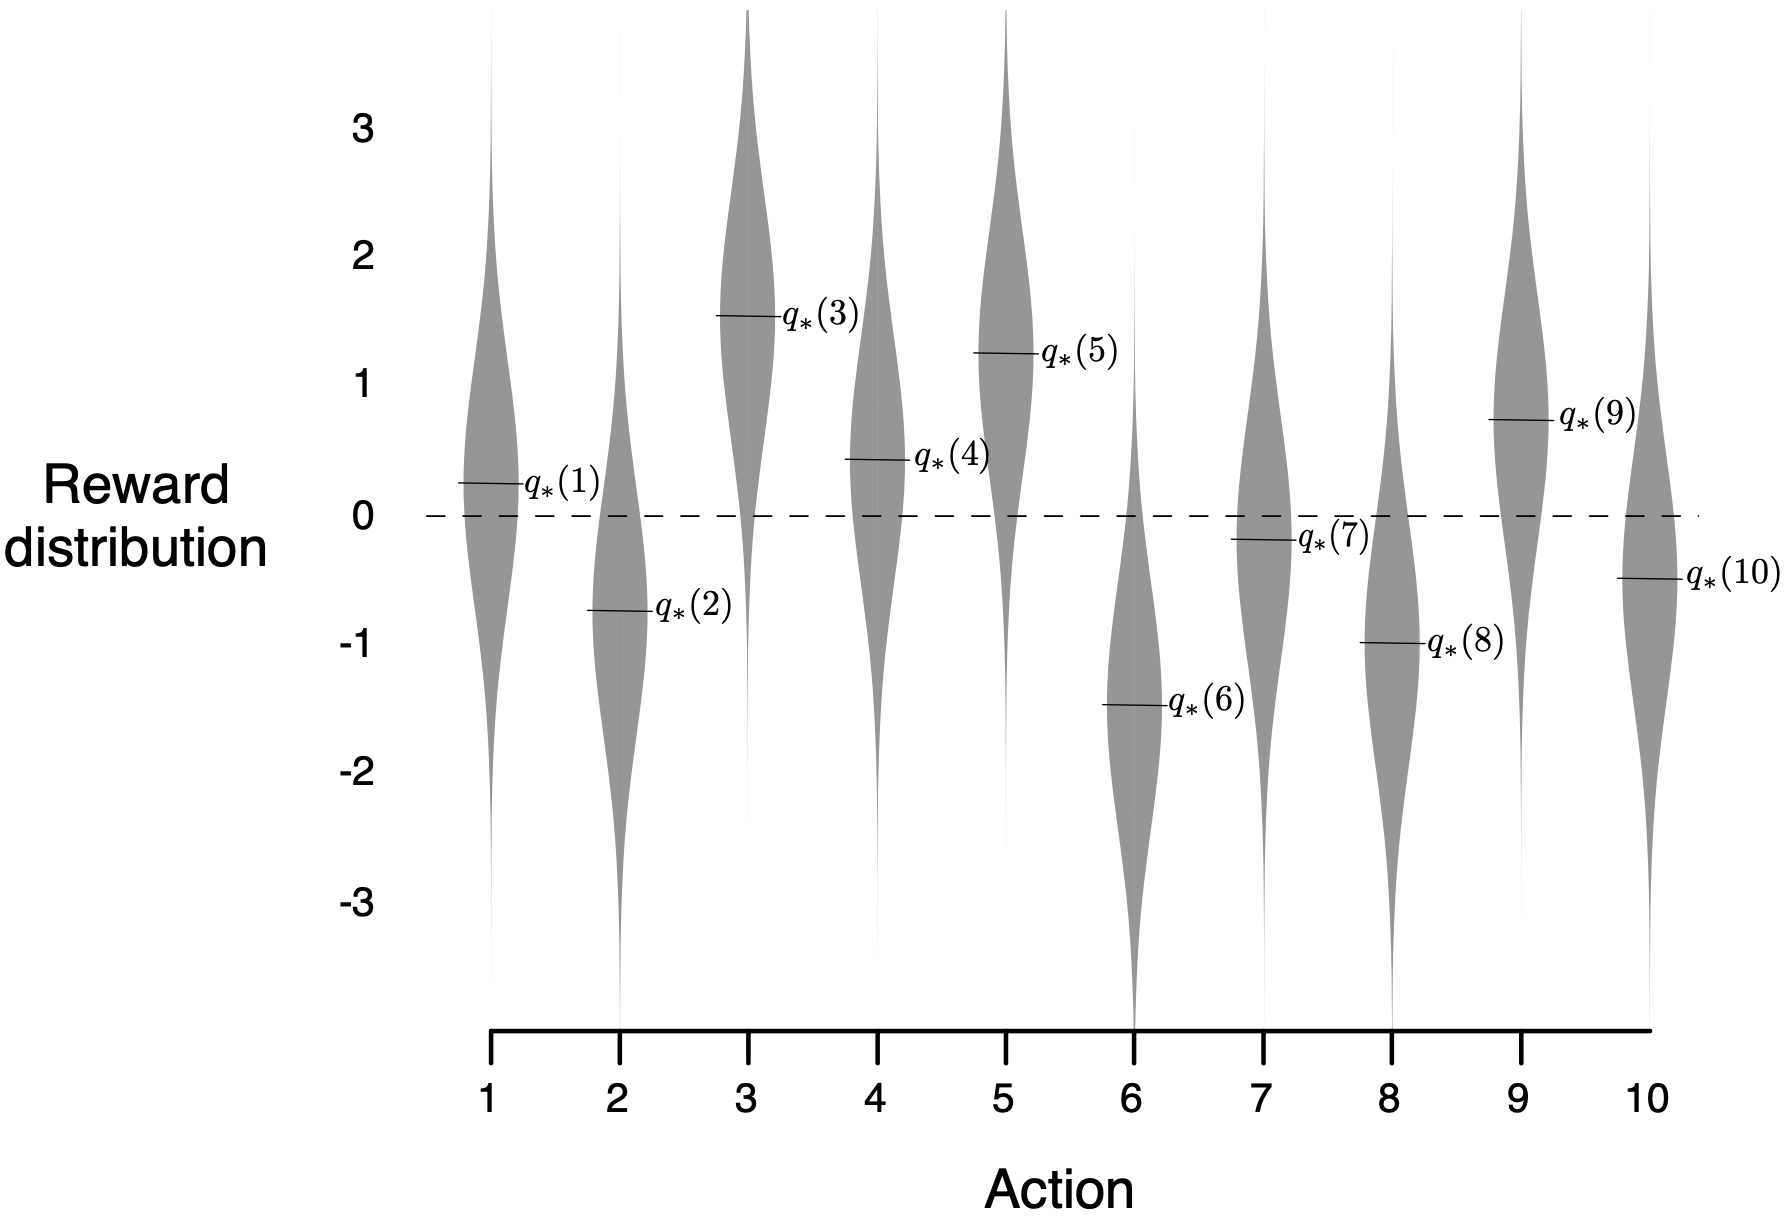
\includegraphics[width=0.9\columnwidth]{images/10-armed-eg1.png}
    \caption{10-armed testbed}
    \label{fig:fig1}
\end{figure}

\begin{itemize}
\item
  \textbf{Figure \ref{fig:fig1}:} An example bandit problem from the 10-armed
  testbed. The true value \(q_*(a)\) of each of the ten actions was
  selected according to a normal distribution with mean zero and unit
  variance, and then the actual rewards were selected according to a
  mean \(q_*(a)\) unit variance normal distribution, as suggested by
  these gray distributions.
\end{itemize}

\begin{itemize}
\item
  Then compares a greedy method with two \(\epsilon\)-greedy methods
  (\(\epsilon = 0.01\) and \(\epsilon = 0.1\)):
\end{itemize}


\begin{figure}[H]
  \centering  % Remember to centre the figure
    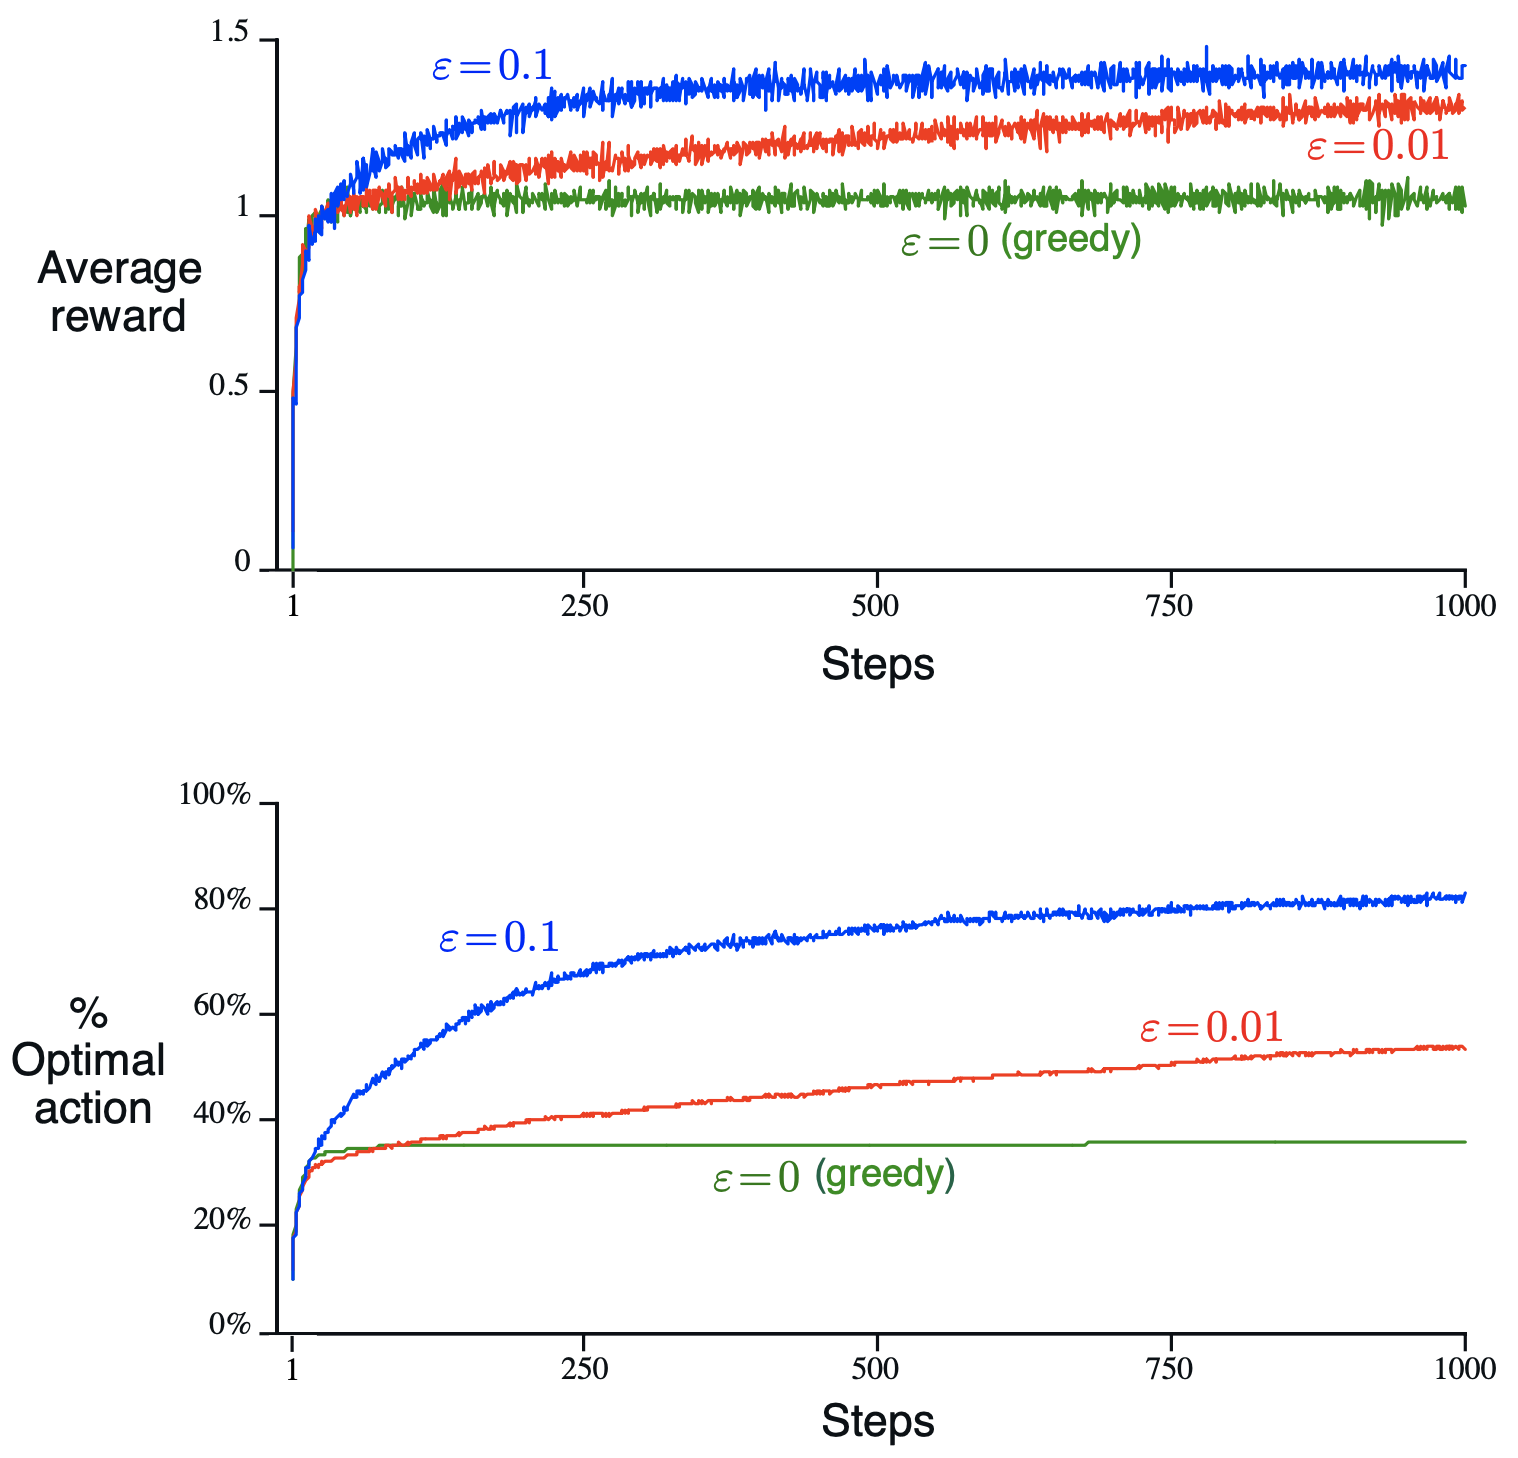
\includegraphics[width=0.9\columnwidth]{images/10-armed-eg2.png}
    \caption{Average performance of \(\epsilon\)-greedy action-value methods on the 10-armed testbed}
    \label{fig:fig2}
\end{figure}


\begin{itemize}
\item
  \textbf{Figure \ref{fig:fig2}:} Average performance of \(\epsilon\)-greedy
  action-value methods on the 10-armed testbed. These data are averages
  over 2000 runs with different bandit problems. All methods used sample
  averages as their action-value estimates.
\end{itemize}

\begin{itemize}
\item
  NOTE:

  \begin{itemize}
  \item
    The \(\epsilon = 0.01\) method improved more slowly, but eventually
    would perform better than the \(\epsilon = 0.1\) method on both
    performance measures shown in the figure.
  \item
    It is \textbf{also possible} to reduce \(\epsilon\) over time to try
    to get the best of both high and low \(\epsilon\) values.
  \item
    With \textbf{noisier rewards} it takes more exploration to find the
    optimal action.
  \end{itemize}
\end{itemize}

\textbf{Exploration} is beneficial even in the deterministic worlds
\textbf{if:}
\begin{itemize}
  \item \textbf{nonstationary} task, that is, the \textbf{true
  values of the actions changed over time} \(\rightarrow\) \textbf{agent's
  decision-making policy changes}.
  \item \textbf{nonstationary} is the case most commonly encountered in reinforcement learning.
\end{itemize}

\textbf{Example:} A simple bandit algorithm

Pseudocode for a complete bandit algorithm using incrementally computed
sample averages and \(\epsilon\)-greedy action selection is shown in the
box below.

\begin{tcolorbox}
  \textbf{Initialize, for \(a = 1 \; to \; k\):} \(\;\;\;\)
  \(Q(a) \leftarrow 0\) \(\;\;\;\) \(N(a) \leftarrow 0\)

  \textbf{Loop forever:}
  $$\;\;\; A \leftarrow \begin{cases} \argmax_{a}Q(a) &\texttt{with probability } 1- \epsilon \;\;\; \texttt{(breaking ties randomly)} \\ \texttt{random action} &\texttt{with probability } \epsilon \end{cases}$$
  $$\;\;\; R \leftarrow bandit(A)$$
  $$\;\;\; N(a) \leftarrow N(a)+1$$
  $$\;\;\; Q(A) \leftarrow Q(A) + \frac{1}{N(A)}[R-Q(A)]$$
\end{tcolorbox}

\begin{itemize}
\item
  Where:

  \begin{itemize}
  \item
    \textbf{function \(bandit(a)\)} is assumed to \textbf{take} an
    action and \textbf{return} a corresponding reward
  \end{itemize}
\end{itemize}









\subsection{Tracking a Nonstationary Problem}\label{tracking-nonstationary-problem}

\textbf{What:} true values of the actions changed over time
\(\rightarrow\) agent's decision-making policy changes.

\textbf{Adjustments:} it makes sense to give more weight to recent
rewards than to long-past rewards.

\begin{itemize}
\item
  A \textbf{POPULAR WAY} it to use a \textbf{constant step-size
  parameter \(\alpha\)} (2.3 modified to be):
\end{itemize}

\begin{gather*}
  Q_{n+1} = Q_n + \alpha [R_n - Q_n] \\ \\
  \textbf{Where:} \\
  \alpha \in (0,1]\ \text{: is constant} \\
\end{gather*}


\textbf{\(\rightarrow\) resulting in \(Q_{n+1}\) being a weighted
average of past rewards and the initial estimate \(Q_1\)} (sometimes
called an \emph{exponential recency-weighted average}):

\[Q_{n+1} = (1 - \alpha )^n Q_1 + \sum_{i=1}^n \alpha (1 - \alpha)^{n-1} R_i \;\;\;\;\;(2.6)\]

\begin{center}\rule{0.5\linewidth}{0.5pt}\end{center}











\subsection{Optimistic Initial Values}\label{optimistic-initial-values}


\textbf{What:} a common strategy of balancing exploration-exploitation.

\textbf{How:} encouraging early exploration with optimistic initial values for all possible actions.

\textbf{Limitations:}
\begin{itemize}
  \item \textcolor{red}{Drive only early exploration}
  \item \textcolor{red}{Not well-suitable for} non-stationary problems
  \item \textcolor{red}{We may not always know how to set the optimistic initial values}, because in practice we may not know the maximal reward.
\end{itemize}














% =============== CHAPTER 3 - Finite Markov Decision Processes ===============



\section{Finite Markov Decision Processes}\label{finite-markov-decision-processes}

\textbf{Markov decision process (MDP)} provides a \uline{mathematical framework
for modeling sequential decision-making in situations where outcomes are partly
random and partly under the control of a decision maker}.

A \textbf{MDP is a 4-tuple \((S,A,p,R)\)}, where:

\begin{itemize}
\item
  \(S\) is a set of states called the state space,
\item
  \(A\) is a set of actions called the action space (alternatively,
  \(A(s)\) is the set of actions available from state \(s\)),
\item
  \(p(s', r|s, a) = Pr\{S_t = s', R_t =r | S_{t-1} = s, A_{t-1} = a\}\)
  is the probability that action \(a\) in state \(s\) at time \(t\) will
  lead to state \(s'\) at time \(t+1\),
\item
  \(R_{a}(s,s')\) is the immediate reward (or expected immediate reward)
  received after transitioning from state \(s\) to state \(s'\), due to
  action \(a\)
\end{itemize}

The state and action spaces may be \textbf{finite} or \textbf{infinite}:

\begin{itemize}
  \item e.g. the set of real numbers is infinite.
  \item Some processes with
  countably infinite state and action spaces can be reduced to ones with
  finite state and action spaces.
\end{itemize}

A \textbf{policy function \(\pi\)} is a (potentially probabilistic)
mapping from state space to action space.

\textbf{Optimization objective} \(\rightarrow\) find a good ``policy''
for the decision maker.

\begin{itemize}
  \item \textbf{EXTRA:} Once a MDP is \textbf{combined
  with} a policy in this way, this fixes the action for each state and the
  resulting combination \textbf{behaves like a Markov chain} (since the
  action chosen in state \(s\) is completely determined by \(\pi(s)\) and
  \(\Pr(s_{t+1}=s'\mid s_{t}=s,a_{t}=a)\) reduces to
  \(\Pr(s_{t+1}=s'\mid s_{t}=s)\), a \textbf{Markov transition matrix}).
\end{itemize}






\subsection{The Agent--Environment Interface }\label{agent-environment-interface}

\textbf{Agent:} learner and decision maker.

\textbf{Environment:} thing agent interacts with, comprising everything
outside the agent.

The environment also gives rise to \textbf{rewards}, special numerical
values that the agent seeks to maximize over time through its choice of
\textbf{actions}.


\begin{figure}[H]
  \centering  % Remember to centre the figure
    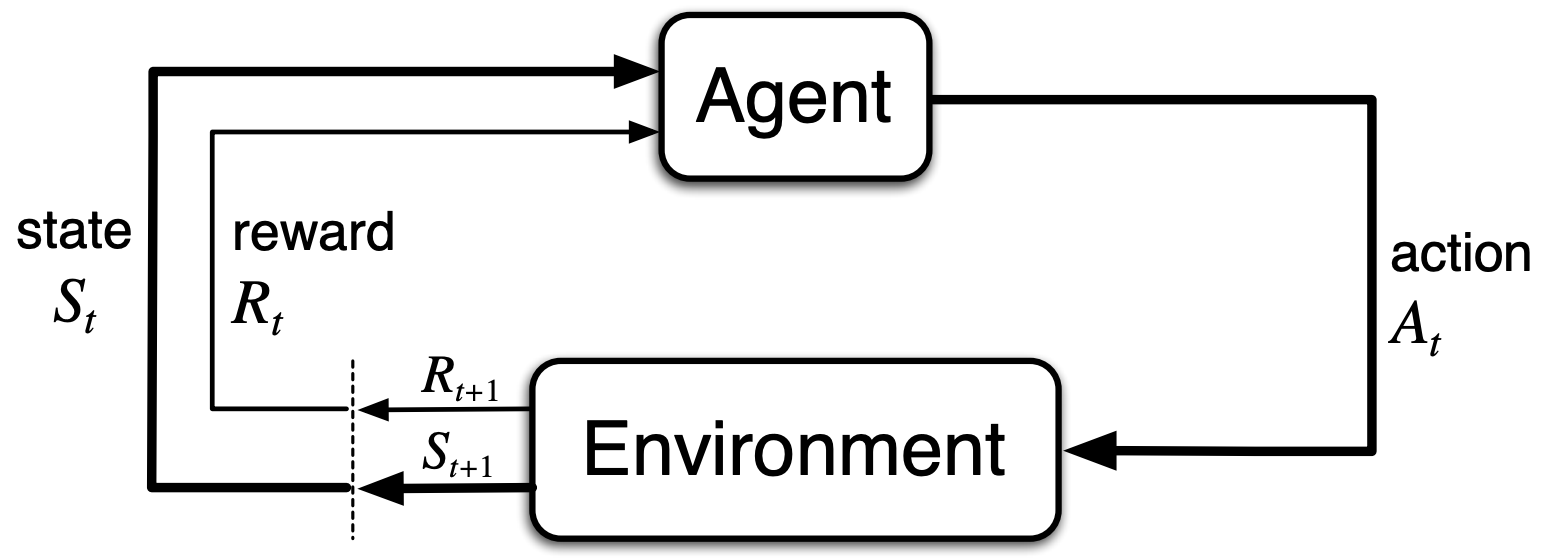
\includegraphics[width=0.9\columnwidth]{images/MDP-agent-environment-interaction.png}
    \caption{MDP agent-environment interaction}
    \label{fig:fig3}
\end{figure}


The MDP and agent together give rise to a \emph{sequence} or
\emph{trajectory} that begins like this:

\[S_0, A_0, R_1, S_1, A_1, R_2, S_2, A_2, R_3,... \]

\emph{In general}, \textbf{actions} can be any decisions we want to
learn how to make, and the \textbf{states} can be anything we can know
that might be useful in making them.

In a \textbf{finite MDP}, the sets of states, actions, and rewards
(\(S\), \(A\), and \(R\)) all have a finite number of elements.

In this case, the \textbf{random variables \(R_t\) and \(S_t\)} have
well defined discrete probability distributions \textbf{dependent only
on} the preceding state and action.

There is a \textbf{probability of those values occurring at time t},
given particular values of the preceding state and action:

\[p(s', r|s, a) = Pr\{S_t = s', R_t =r | S_{t-1} = s, A_{t-1} = a\},\]

Where:

\begin{itemize}
\item
  \(s' =\) particular values of the random variable \(S\) (\(s' \in S\))
\item
  \(r =\) particular values of the random variable \(R\) (\(r \in R\))
\end{itemize}

The \textbf{function \(p\)} defines the dynamics of the MDP. \(p\)
specifies a probability distribution for each choice of \(s\) and \(a\).

Total probability is thus:

\[\sum_{s' \in S} \sum_{r \in R} p(s', r|s, a) = 1, for\;all\;s \in S, a \in A(s)\]

\textbf{Markov property:} The state must include information about all
aspects of the past agent--environment interaction that make a
difference for the future.

\begin{itemize}
  \item (only present matters)
  \item (things/rules/transition model are stationary)
  \item We will assume the
  Markov property throughout this book.
\end{itemize}


\textbf{Calculations from the four-argument dynamics function:}

\begin{itemize}
\item
  \textbf{state-transition probabilities
  \(p : S \times S \times A \rightarrow [0, 1]\)}

  \begin{itemize}
  \item
    \(p(s'|s, a) = Pr\{S_t = s'| S_{t-1} = s, A_{t-1} = a\} = \sum_{r \in R} p(s', r|s, a)\)
  \end{itemize}
\item
  \textbf{expected rewards for state--action pairs
  \(r : S \times A \rightarrow \mathbb{R}\)}

  \begin{itemize}
  \item
    \(r(s,a) = E[R_t | S_{t-1}=s, A_{t-1}=a] = \sum_{r \in R} \sum_{s' \in S} p(s', r|s, a)\)
  \end{itemize}
\item
  \textbf{expected rewards for state--action--next-state triples
  \(r : S \times A \times S \rightarrow \mathbb{R}\)}

  \begin{itemize}
  \item
    \(r(s,a, s') = E[R_t | S_{t-1}=s, A_{t-1}=a, S_t = s'] = \sum_{r \in R} r \frac{p(s', r | s, a)}{p(s' | s, a)}\)
  \end{itemize}
\end{itemize}









\subsection{Goals and Rewards}\label{goals-and-rewards}

\textbf{Reward Hypothesis:}

\begin{itemize}
\item
  That all of what we mean by \textbf{goals $G$} and purposes \emph{can be well thought of as} the \uline{maximization of the expected value of the cumulative sum of a received scalar signal (called reward)}.
\end{itemize}

It is critical that the rewards we set up truly indicate what we want
accomplished.

\begin{itemize}
  \item \textbf{For example}, a chess-playing agent should be
  rewarded only for actually winning, not for achieving subgoals such as
  taking its opponent's pieces or gaining control of the center of the
  board. If achieving these sorts of subgoals were rewarded, then the
  agent might find a way to achieve them without achieving the real goal.
\end{itemize}

\textbf{Reward signal} is your way of communicating to the robot what
you want it to achieve, not how you want it achieved.







\subsection{Returns and Episodes }\label{returns-and-episodes}

In general, we seek to maximize the expected \textbf{return}, where the
return, denoted \(G_t\).

\textbf{Episodic Tasks}\label{episodic-tasks}

\(G_t\) is in the simplest case the \textbf{return} of the sum of the
rewards:

\[G_t \dot{=} R_{t+1} + R_{t+2} + R_{t+3} + ... + R_T \;\;\;\;\;(3.7)\]

Tasks with \emph{episodes} of this kind are called \textbf{episodic
tasks}. In episodic tasks we \textbf{sometimes need to distinguish} the
set of all nonterminal states, denoted \(S\), from the set of all states
plus the terminal state, denoted \(S^+\). The time of termination,
\(T\), is a random variable that normally varies from episode to
episode.


\textbf{Continuing Tasks}\label{continuing-tasks}


On the other hand, in many cases the agent--environment interaction does
not break naturally into identifiable episodes, but goes on
\textbf{continually without limit}. We call these \textbf{continuing
tasks}.

In this book we usually use a definition of return that is slightly more
complex conceptually but much simpler mathematically. The additional
concept that we need is that of \textbf{discounting}. According to this
approach, the agent tries to select actions so that the sum of the
discounted rewards it receives over the future is maximized. In
particular, it chooses \(A_t\) to maximize the expected discounted
return:

\[G_t = R_{t+1} + \gamma R_{t+2} + \gamma^2 R_{t+3} + ... = \sum_{k=0}^{\infty} \gamma^k R_{t+k+1} \;\;\;\;\;(3.8)\]

Where:

\begin{itemize}
\item
  \(\gamma =\) is a parameter, \(0 \leq \gamma \leq 1\), called the
  \textbf{discount rate}.

  \begin{itemize}
  \item
    If \(\gamma < 1\), the infinite sum has a finite value as long as
    the reward sequence \(\{R_k\}\) is bounded.
  \item
    If \(\gamma = 0\), the agent is ``myopic'' in being concerned only
    with maximizing immediate rewards: its objective in this case is to
    learn how to choose \(A_t\) so as to maximize only \(R_{t+1}\). But
    in general, acting to maximize immediate reward can reduce access to
    future rewards so that the return is reduced.
  \item
    As \(\gamma\) approaches \(1\), the return objective takes future
    rewards into account more strongly; the agent becomes more
    farsighted.
    \begin{itemize}
      \item If $\gamma = 1$, undiscounted.
    \end{itemize}
  \end{itemize}
\end{itemize}

\textbf{Returns at successive time steps} are related to each other in a
way that is important for the theory and algorithms of reinforcement
learning:

\begin{align*}
  G_t &= R_{t+1} + \gamma R_{t+2} + \gamma^2 R_{t+3} + \gamma^3 R_{t+4} + ... \\
  &= R_{t+1} + \gamma (R_{t+2} + \gamma R_{t+3} + \gamma^2 R_{t+4} + ...)  \\
  &= R_{t+1} + \gamma G_{t+1} \\
\end{align*}

\begin{itemize}
\item
  Note that this works for all time steps \(t<T\), even if termination
  occurs at \(t + 1\), if we define \(G_T = 0\)
\item
  Note that although the return is a sum of an infinite number of terms,
  it is still finite if the reward is nonzero and constant, if
  \(\gamma < 1\).
\end{itemize}






\subsection{Unified Notation for Episodic and Continuing Tasks}
\label{unified-notation-for-episodic-and-continuing-tasks}

In the preceding section we described two kinds of reinforcement
learning tasks:

\begin{itemize}
\item
  \textbf{episodic tasks:} agent--environment interaction naturally
  breaks down into a sequence of separate episodes.
\item
  \textbf{continuing tasks:} agent--environment interaction don't breaks
  down into a sequence of separate episodes.
\end{itemize}

We have defined the return as a sum over a finite number of terms in one
case (3.7) and as a sum over an infinite number of terms in the other
(3.8). These two can be unified by considering \textbf{episode
termination} to be the entering of a \uline{special absorbing state that
transitions only to itself and that generates only rewards of zero}. For
example, consider the state transition diagram:


\begin{figure}[H]
  \centering  % Remember to centre the figure
    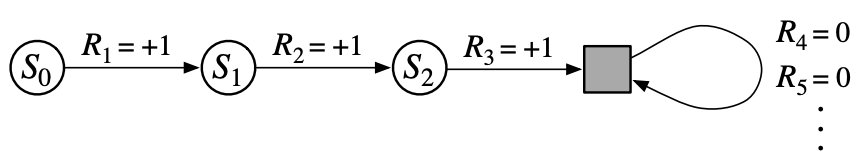
\includegraphics[width=0.9\columnwidth]{images/Unified-Notation-Episodic-and-Continuing-Tasks.png}
    \caption{State transition diagram}
    \label{fig:fig4}
\end{figure}


Starting from \(S_0\), we get the reward sequence
\(+1, +1, +1, 0, 0, 0,...\). Summing these, we get the same return
whether we sum over the first \(T\) rewards (here \(T = 3\)) or over the
full infinite sequence. This remains true even if we introduce
discounting.

Thus, we can define the \textbf{return, in general}, according to (3.8),
using the convention of omitting episode numbers when they are not
needed, and including the possibility that = 1 if the sum remains
defined (e.g., because all episodes terminate). Alternatively, we can
write:

\[G_t = \sum_{k=t+1}^T \gamma^{k-t-1} R_k\]

\begin{itemize}
\item
  including the possibility that \(T = \infty\) or \(\gamma = 1\) (but
  not both).
\end{itemize}







\subsection{Policies and Value Functions}\label{policies-and-value-functions}

Almost all \textbf{reinforcement learning algorithms involve estimating
\textcolor{blue}{value functions}} --- functions of states (or of state--action
pairs) that \uline{estimate how good it is for the agent to be in a given state} (or \uline{how good it is to perform a given action in a given state}). They allow an agent to query the quality of its current situation instead of waiting to observe the long-term outcome. Thus, \uline{\textbf{value functions} enable us to judge the quality of different \textbf{policies}}.

\begin{figure}[H]
  \centering  % Remember to centre the figure
    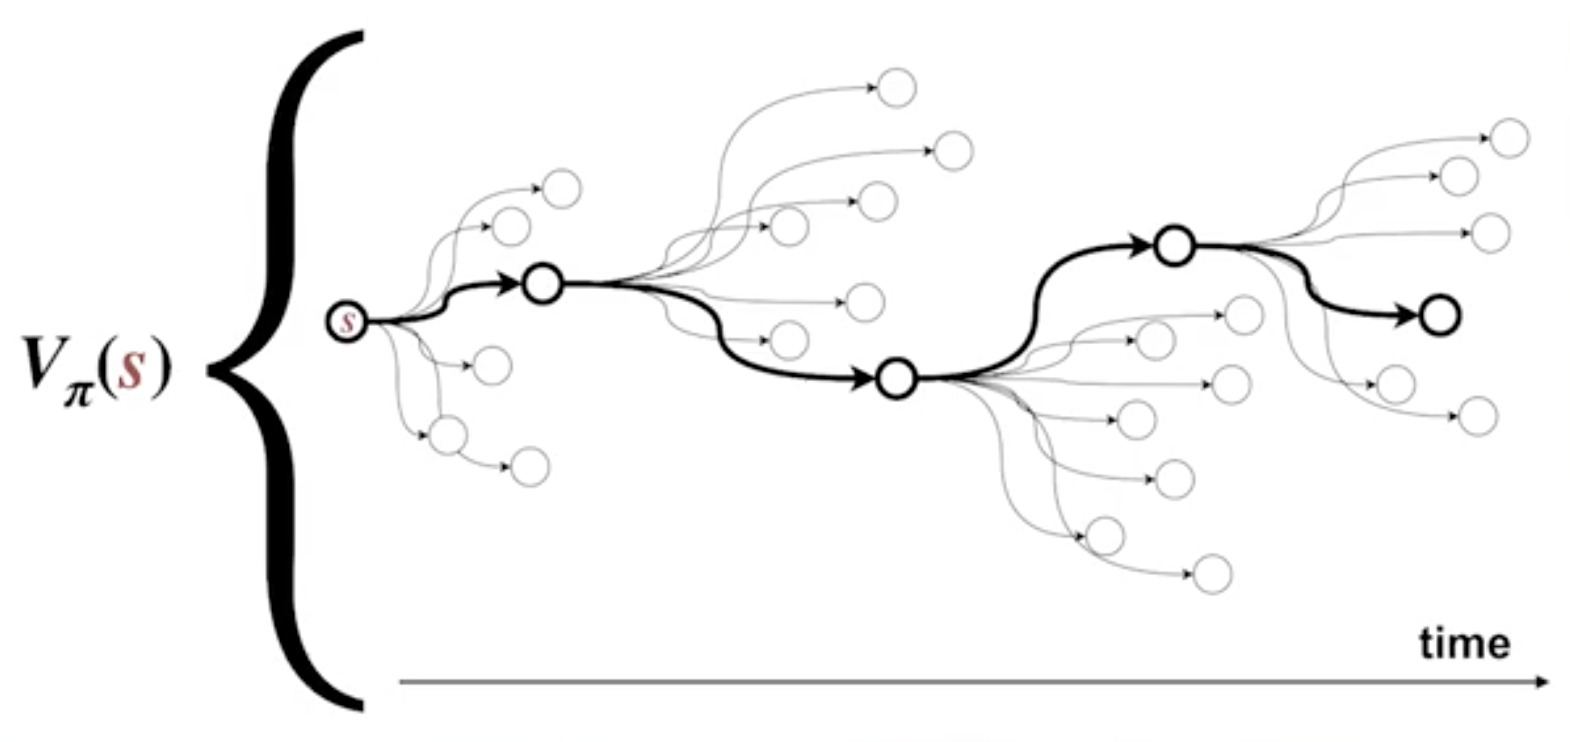
\includegraphics[width=0.8\columnwidth]{images/value-function-predicting-rewards.png}
    \caption{Illustration of value function predicting rewards into the future}
    \label{fig:value-function-predicting-rewards}
\end{figure}

\textcolor{blue}{\textbf{Policy \(\pi\)}} is a \uline{\textbf{mapping from} states \textbf{to} probabilities of selecting each possible action}. If the agent is
following policy \(\pi\) at time \(t\), then \(\pi(a|s)\) is the
probability that \(A_t = a\) if \(S_t = s\).

A policy by definition \uline{depends only on the current state}. It cannot depend on things like time or previous states. This is best thought of as a restriction on the state, not the agent. The state should provide the agent with all the information it needs to make a good decision.

\begin{itemize}
  \item Accordingly, value functions are defined with respect to particular ways of acting, called \textbf{policies}.
\end{itemize}

\begin{figure}[H]
  \centering  % Remember to centre the figure
    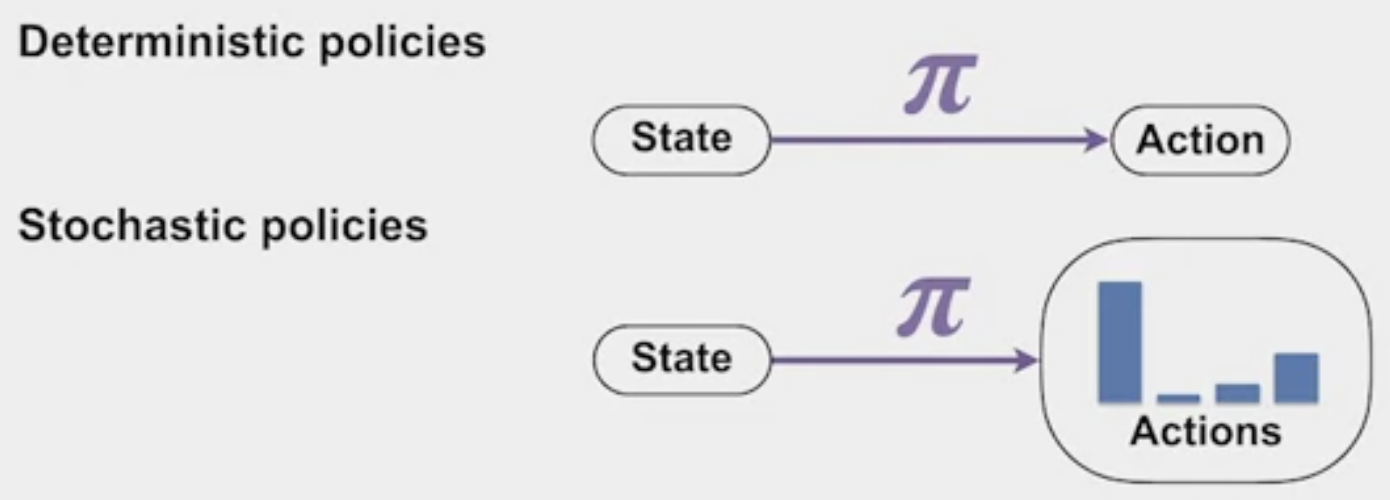
\includegraphics[width=0.8\columnwidth]{images/deterministic-and-stochastic-policies.png}
    \caption{Policies tell an agent how to behave in their environment}
    \label{fig:value-function-predicting-rewards}
\end{figure}

\textbf{Reinforcement learning methods specify} \uline{how the agent's policy is changed as a result of its experience}.

The \textcolor{blue}{\textbf{state-value functions \(v_\pi(s)\)}} of a state \(s\) under a policy \(\pi\), is the expected return when starting in \(s\) and following \(\pi\) thereafter. For MDPs, we can define \(v_\pi\) formally by

\[v_\pi(s) = E_\pi[G_t|S_t=s] = E_\pi[\sum_{k=0}^{\infty} \gamma^k R_{t+k+1} | S_t = s], for\;all\; s \in S \;\;\;\;\;(3.12)\]

Where:

\begin{itemize}
\item
  \(E_\pi[]\) denotes the expected value of a random variable given that
  the agent follows policy \(\pi\), and \(t\) is any time step.
\end{itemize}

The \textcolor{blue}{\textbf{action-value function \(q_\pi(s, a)\)}} for policy \(\pi\) is
defined as the \textbf{value of taking action \(a\) in state \(s\) under
a policy \(\pi\)}, as the expected return starting from \(s\), taking
the action \(a\), and thereafter following policy \(\pi\):

\[q_\pi(s, a) = E_\pi[G_t|S_t=s, A_t=a] = E_\pi[\sum_{k=0}^{\infty} \gamma^k R_{t+k+1} | S_t = s, A_t = a] \;\;\;\;\;(3.13)\]

A \textbf{fundamental property of value functions} used throughout
reinforcement learning and dynamic programming is that they satisfy
recursive relationships similar to that which we have already
established for the return (3.9).








\subsection{Optimal Policies and Value Functions}\label{optimal-policies-and-value-functions}

\textcolor{Green}{\textbf{Solving a reinforcement learning task}} means, roughly, finding a policy that achieves a lot of reward over the long run.

For finite MDPs, we can precisely define an \textcolor{blue}{\textbf{optimal policy \(\pi_*\)}} as follows: * \(\pi \geq \pi'\) if and only if
\(v_\pi(s) \geq v_{\pi'}(s)\) for all \(s \in S\) * \textbf{Always at
least one policy} that is better than or equal to all other policies.


\begin{figure}[H]
  \centering  % Remember to centre the figure
    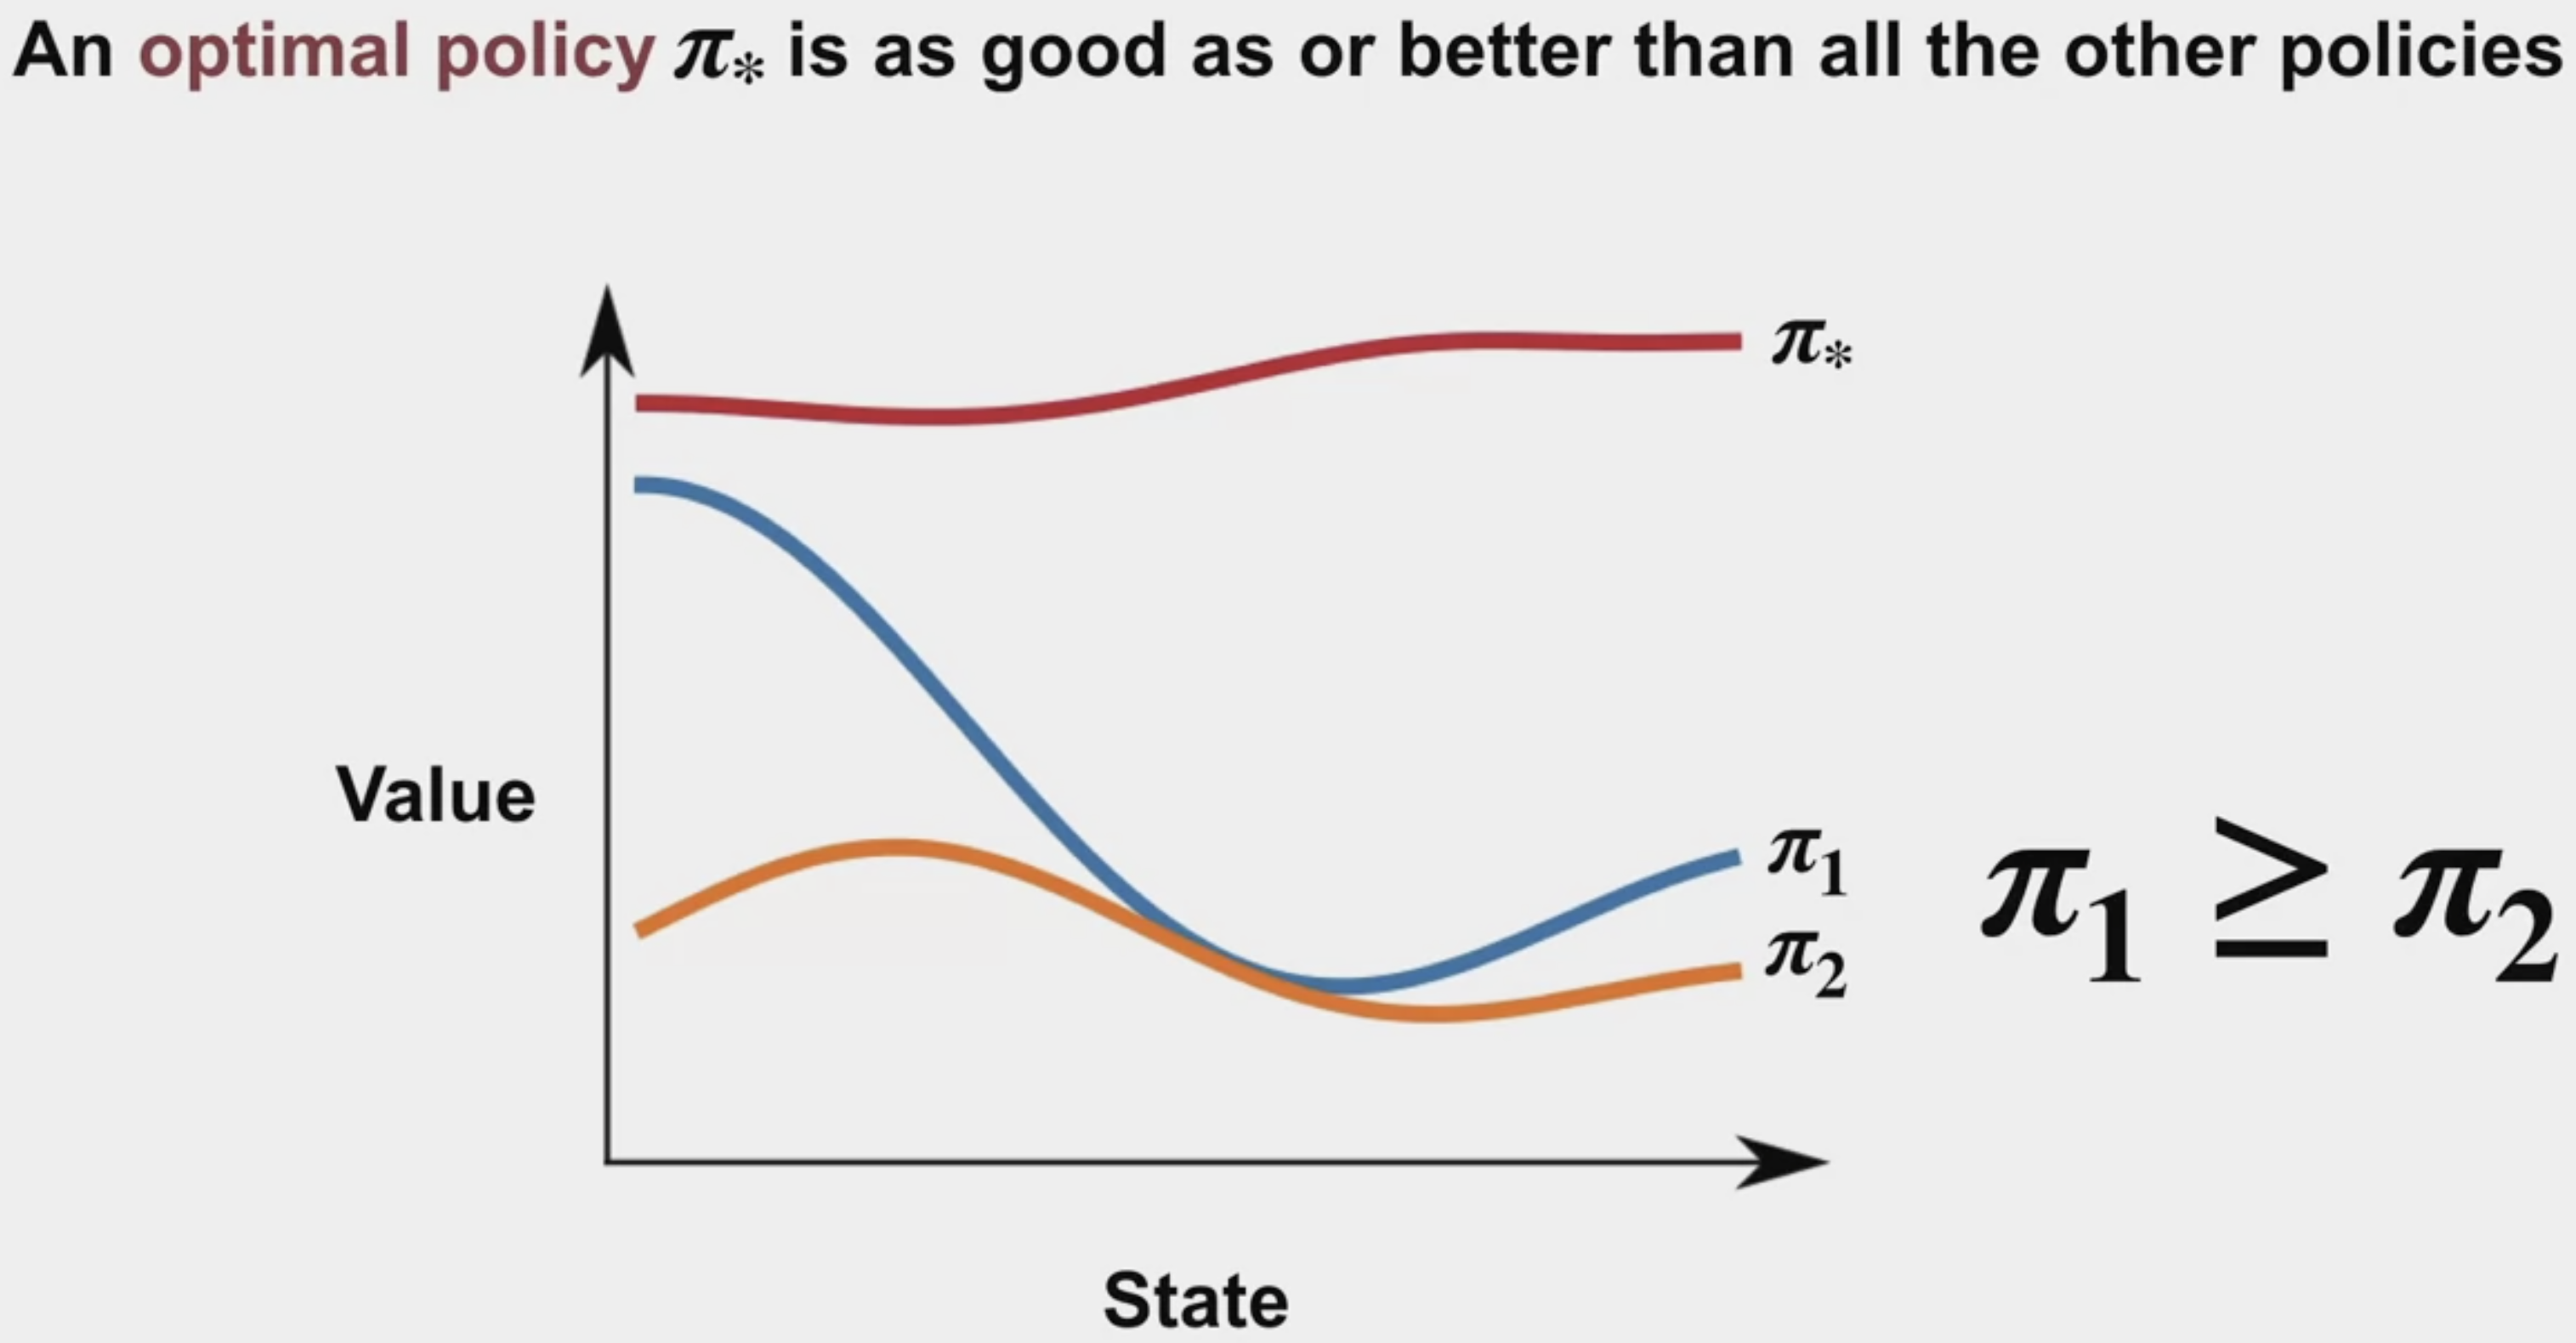
\includegraphics[width=0.8\columnwidth]{images/optimal-policy-eg.png}
    \caption{Illustration of optimal policy}
    \label{fig:optimal-policy-eg}
\end{figure}

How to find an optimal policy:
\begin{itemize}
  \item Once we had the \uline{optimal state value function}, it's relatively easy to work out the optimal policy.
  \item If we have the \uline{optimal action value function}, working out the optimal policy is even easier.
\end{itemize}

All optimal policies share the same \textcolor{blue}{\textbf{optimal state-value function
\(v_*\)}} defined as:

\[v_*(s) = \max_\pi v_\pi(s) \;for\;all\; s \in S \;\;\;\;\;\;(3.15)\]

Optimal policies also share the same \textcolor{blue}{\textbf{optimal action-value function \(q_*\)}} defined as:

\[q_*(s, a) = \max_\pi q_\pi(s, a) \;for\;all\; s \in S \; \& \; a \in A(s) \;\;\;\;\;\;(3.16)\]

For the state--action pair \((s, a)\), this function gives the expected
return for taking action \(a\) in state \(s\) and thereafter following
an optimal policy. Thus, we can write \textbf{\(q_*\) in terms of
\(v_*\)} as follows \textbf{(Bellman equation)}:

\[q_*(s, a) = E[R_{t+1} + \gamma v_*(S_{t+1}) | S_t = s, A_t = a] \;\;\;\;\;\;(3.17)\]






\subsection{Optimality and Approximation }\label{optimality-and-approximation}

For the kinds of tasks in which we are interested, \textcolor{red}{optimal policies can be generated only with extreme computational cost}. In particular, the amount of computation it can perform in a single time step.







\subsection{Why Bellman equations}\label{why-bellman-equations}

\textcolor{blue}{\textbf{Bellman equations}} define a \textbf{relationship between} the \uline{value of a state} or state-action pair and its \uline{possible successor states}.


Consider:

\begin{itemize}
  \item \textbf{Environment:}
  \begin{itemize}
    \item 4 states (A, B, C, D) in a square gridworld
    \item 25\% probability of moving (up, down, left or right)
    \begin{itemize}
      \item bumping into a border will result into staying in the current state
    \end{itemize}
  \end{itemize}
  \item \textbf{Policy:} Uniform random policy
  \item \textbf{Rewards:} The reward is 0 everywhere except for any time the agent lands in state B, the reward is +5.
  \item \textbf{Discoun factor $\gamma$:} 0.7
\end{itemize}

For the given setup, we can write value functions for each of the states (A, B, C, D) in form of Bellman equations:

\begin{figure}[H]
  \centering  % Remember to centre the figure
    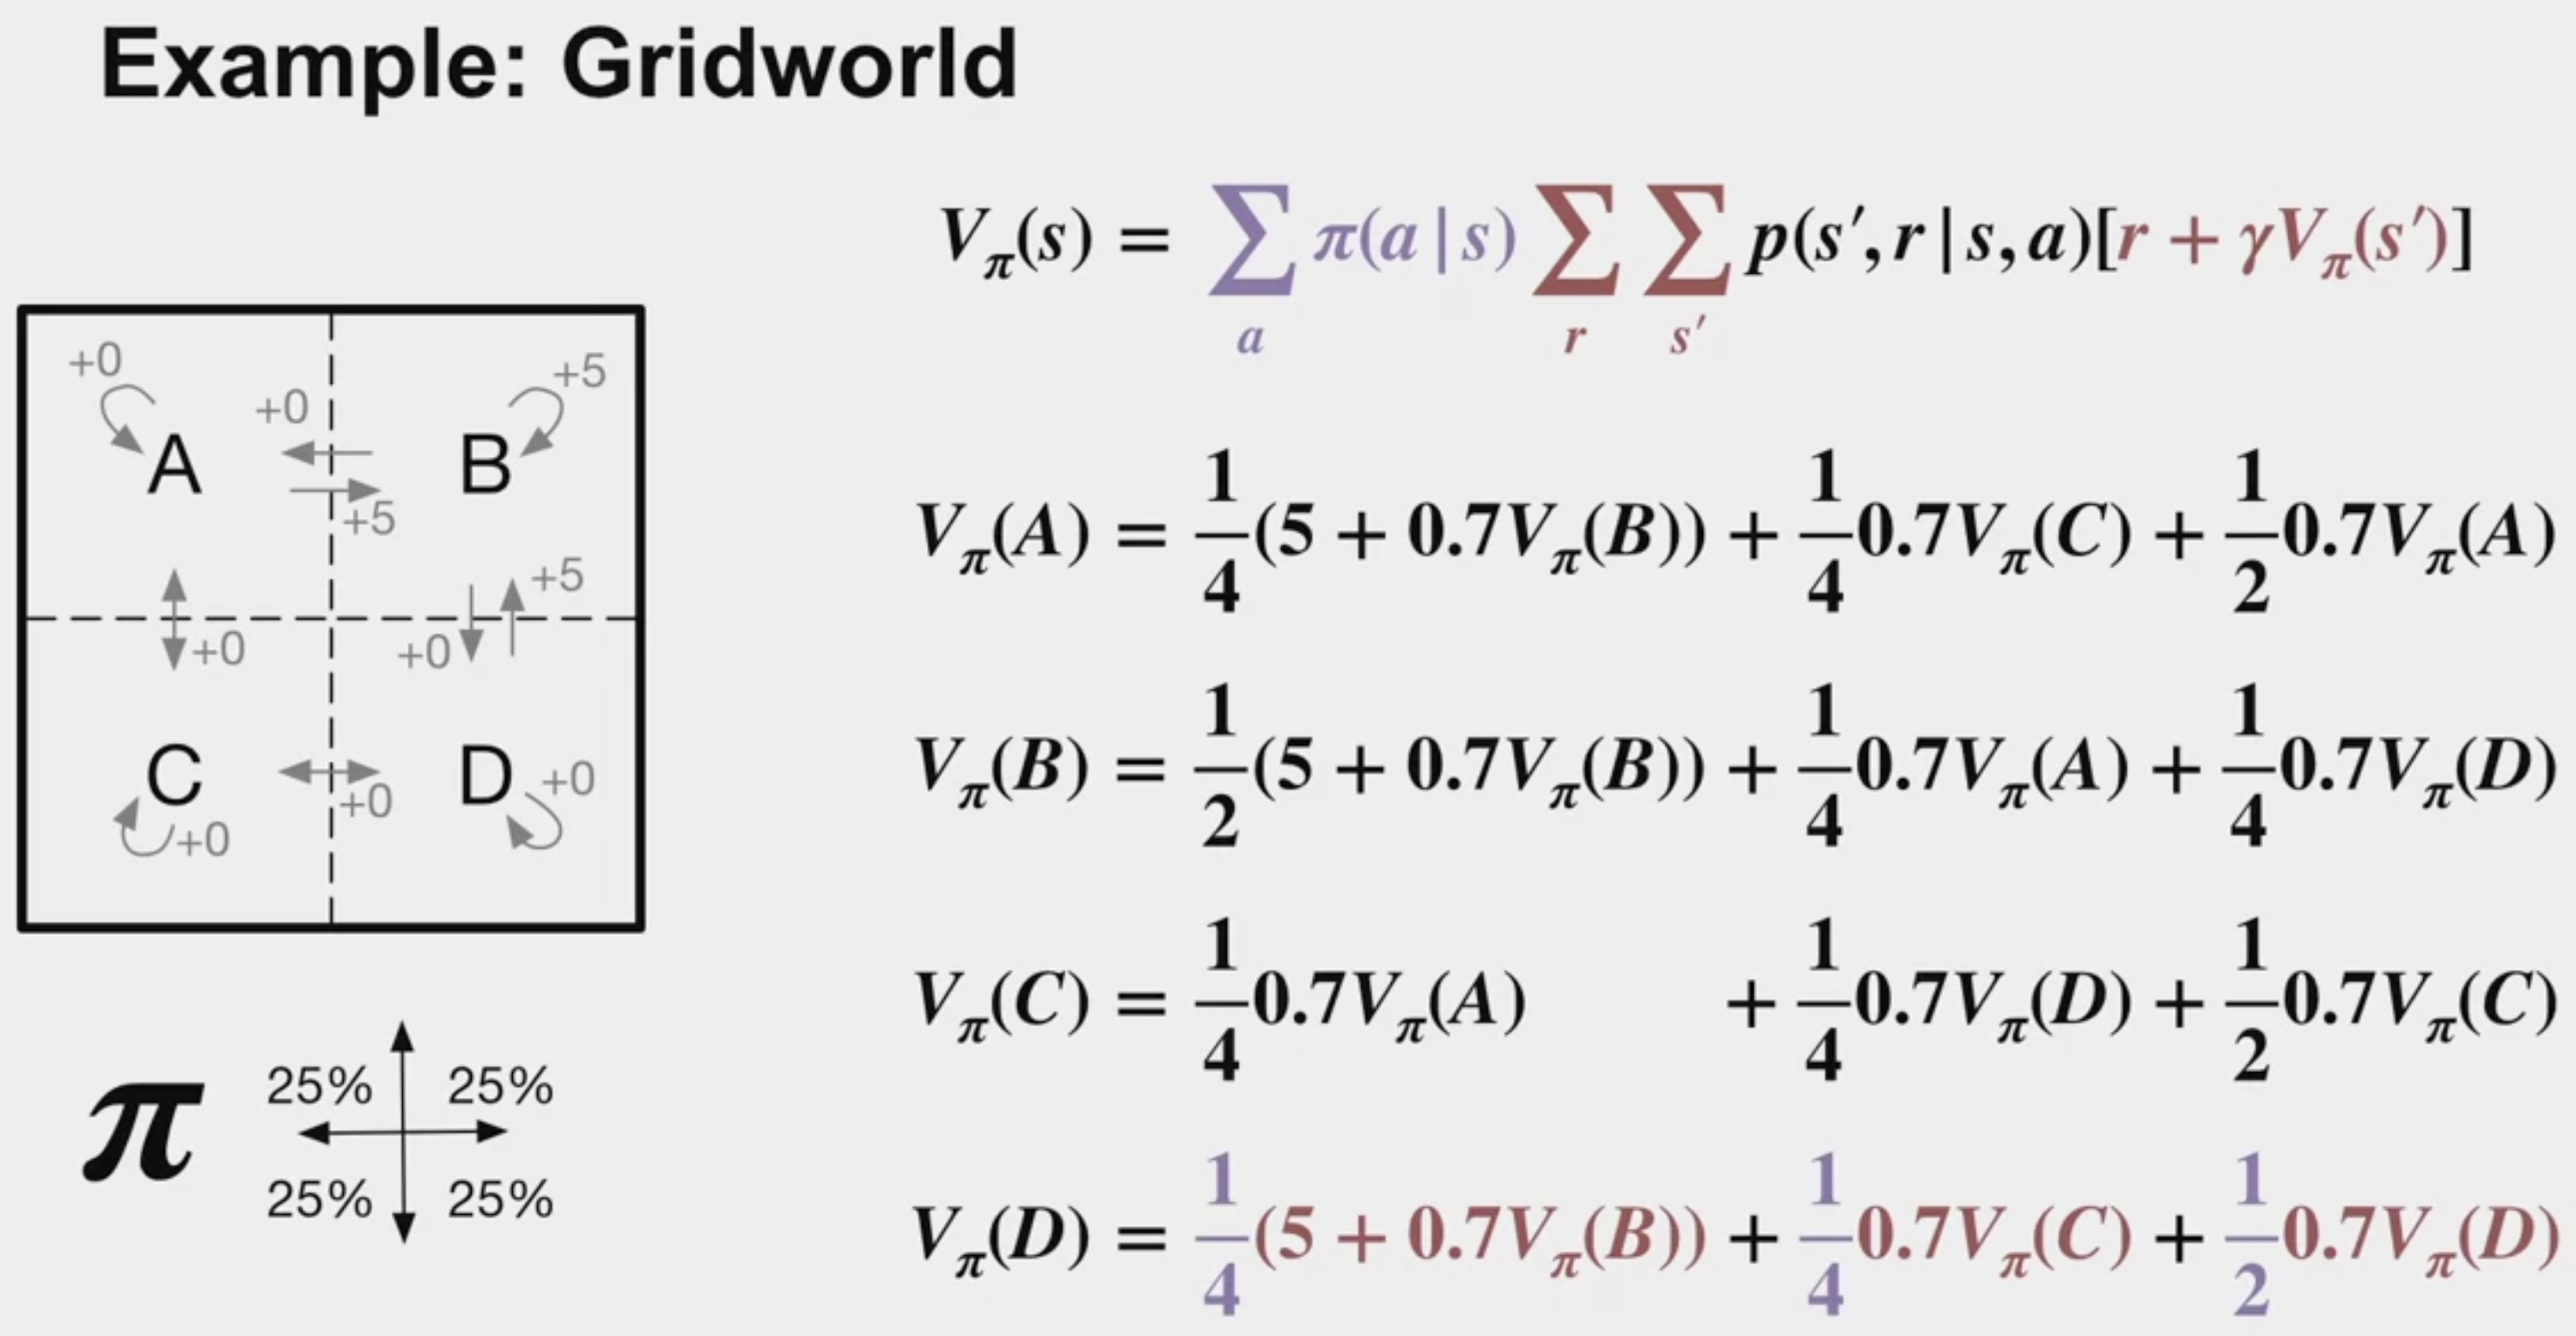
\includegraphics[width=0.9\columnwidth]{images/gridworld-eg.png}
    \caption{Value functions for all gridworld states}
    \label{fig:gridworld-eg}
\end{figure}
\begin{itemize}
  \item \textbf{Unique solutions to the Bellman equations:}
  \begin{itemize}
    \item $V_\pi(A) = 4.2$
    \item $V_\pi(B) = 6.1$
    \item $V_\pi(C) = 2.2$
    \item $V_\pi(D) = 4.2$
  \end{itemize}
\end{itemize}

The \textbf{important thing to note} is that the \uline{Bellman equation reduced an unmanageable infinite sum over possible futures, to a simple linear algebra problem}.

In this case we used the \textbf{Bellman equation} \uline{to directly write down a system of equations for the state values, and then some the system to find the values}. This approach may be possible for MDPs of moderate size. However, \textcolor{Red}{in more complex problems, this won't always be practical}.

\begin{itemize}
  \item e.g. Consider the game of chess for example. We probably won't be able to even list all the possible states, there are around 10 to the 45 of them.

  \begin{figure}[H]
    \centering  % Remember to centre the figure
      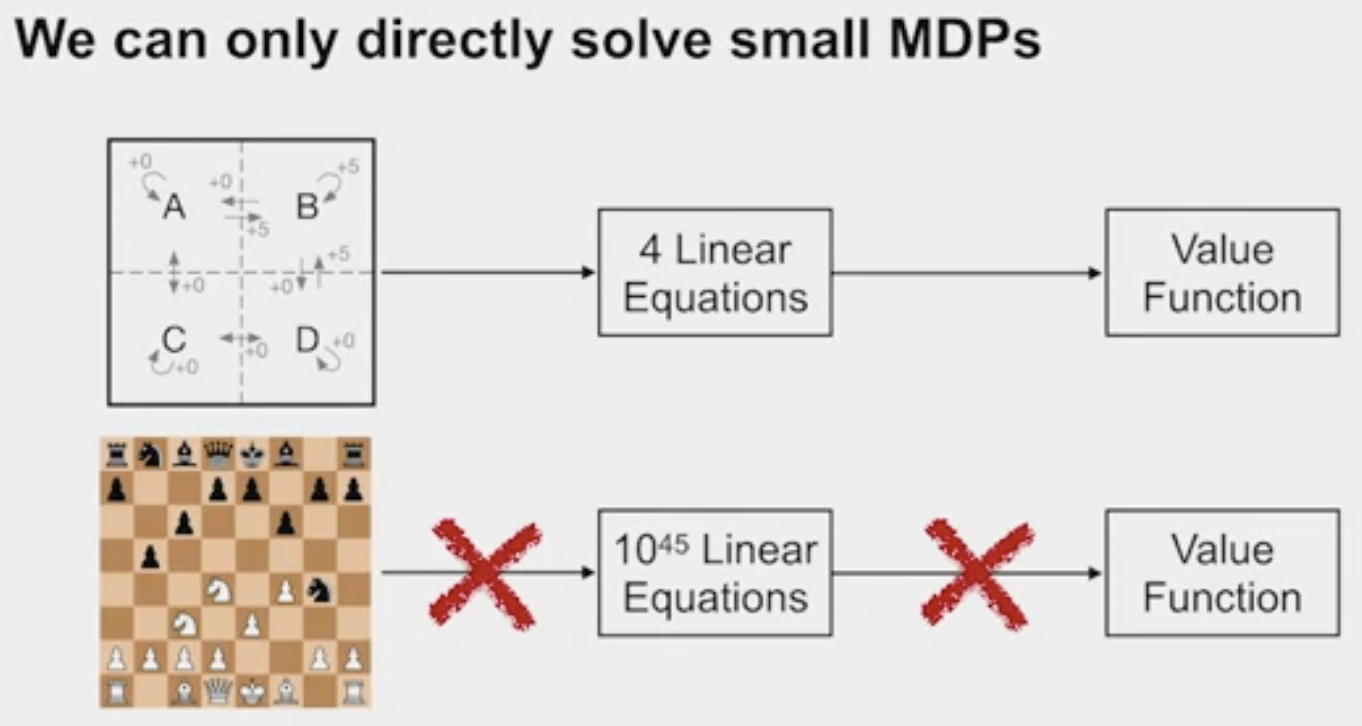
\includegraphics[width=0.8\columnwidth]{images/gridworld-eg2.png}
      \caption{Illustration how directly solving MDPs gets quickly problematic}
      \label{fig:gridworld-eg}
  \end{figure}

\end{itemize}




\subsection{Summary}\label{summary}

\textcolor{Green}{\textbf{Solving a reinforcement learning task}} means, roughly, finding a policy that achieves a lot of reward over the long run.

The \textbf{first step in applying reinforcement learning} will always be to \uline{formulate the problem as an MDP}.

\textcolor{blue}{\textbf{Markov property:}} The state must include information about all aspects of the past agent--environment interaction that make a
difference for the future.
\begin{itemize}
  \item (only present matters)
  \item (things/rules/transition model are stationary)
  \item We will assume the
  Markov property throughout this book.
\end{itemize}

\textcolor{blue}{\textbf{Policy \(\pi\), \(\pi(a|s)\):}} action to take for any given
state

\begin{itemize}
  \item Any policy: \(\pi(s) \rightarrow a\)
  \item Optimal policy:
  \(\pi^*(s) \rightarrow a\) * maximizes long-term expected reward
\end{itemize}


\textcolor{blue}{\textbf{State-Value functions \(v_\pi(s)\):}} expected cumulative rewards
when starting in \(s\) and following policy \(\pi\) thereafter.

\begin{itemize}
  \item or MDPs, we can define \(v_\pi\) formally by
  $$v_\pi(s) = E_\pi[G_t|S_t=s]$$

  \item \textbf{State-Value functions \(v_\pi(s)\):} can be decomposed into \textbf{immediate} and \textbf{future} components using \textcolor{blue}{\textbf{Bellman equation}}. Bellman equation forms the basis of a number of ways to compute, approximate, and learn \(v_\pi\).
  \begin{align*}
  V(s) &= E[G_t | s_t = s] \\
  V(s) &= E[r_{t+1} + \gamma V(s_{t+1} | s_t = s)] \\
  \end{align*}
  \begin{gather*}
    \textbf{Where:} \\
    \gamma =: \text{ is a parameter, \(0 \leq \gamma \leq 1\), called the
    \textbf{discount rate}.} \\
    \text{When \(0\) \(\rightarrow\) consider only
    immediate rewards} \\
    \text{When approaches \(1 \rightarrow\) forward looking}
  \end{gather*}
\end{itemize}

\textcolor{blue}{\textbf{Action-Value functions \(q_\pi(s, a), Q_\pi\):}} expected cumulative reward of taking action \(a\) when starting in \(s\) and
following policy \(\pi\) thereafter.
$$q_\pi(a) = E[R_t | A_t = a]$$

\begin{itemize}
  \item \textbf{Action-Value functions \(v_\pi(s)\):} can also be decomposed
  into \textbf{immediate} and \textbf{future} components using
  \textcolor{blue}{\textbf{Bellman equation}}.
  $$Q_\pi(s,a) = E_\pi[r_t + \gamma Q_\pi (S_{t+1}, a_{t+1}) | s_t=s, a_t=a]$$
  $$Q_\pi(s,a) = \sum_{s'} T(s,a,s') r(s,a,s') + \gamma \sum_{s'}T(s,a,s')Q_\pi(s',\pi(s'))$$
\end{itemize}

\textcolor{blue}{\textbf{Return \(G\) \& Rewards \(R\):}} return is the total of rewards

\begin{itemize}
  \item \(R(s) =\) reward of \textbf{entering state \(s\)}
  \item \(R(s, a) =\) reward of \textbf{entering state \(s\)} \& \textbf{taking action \(a\)}
  \item \(R(s, a, s') =\) reward of \textbf{being in state \(s\)} \& \textbf{taking action \(a\)} \& \textbf{entering state \(s'\)}
\end{itemize}

\textcolor{blue}{\textbf{State \(S\):}} every state agent could be in

\begin{itemize}
  \item \(S =\) set of \textbf{nonterminal states}
  \begin{itemize}
    \item \(s' =\) particular values of the random variable \(S\) (\(s' \in S\))
  \end{itemize}
  \item \(S^+ =\) set of \textbf{terminal states}
\end{itemize}

\textcolor{blue}{\textbf{Actions \(A, A(s)\):}} every action agent could take

\textcolor{blue}{\textbf{Function \(p\) (a.k.a Model / Transition function):}} defines the
dynamics of the environment. \(p\) specifies a probability distribution
for each choice of \(s\) and \(a\).

\begin{itemize}
  \item \textbf{state-transition
  probabilities \(p : S \times S \times A \rightarrow [0, 1]\)}
  $$
  p(s'|s, a) = Pr\{S_t = s'| S_{t-1} = s, A_{t-1} = a\} = \sum_{r \in R} p(s', r|s, a)
  $$
\end{itemize}

\begin{center}\rule{0.5\linewidth}{0.5pt}\end{center}












% =============== CHAPTER 4 - Dynamic Programming ===============


\section{Dynamic Programming (DP)}\label{dynamic-programming}


\textbf{What:} refers to a \uline{collection of algorithms that can be used to \textbf{compute optimal policies} given a perfect model of the environment as a Markov decision process (MDP)}.


Pros and cons:

\begin{itemize}
  \item \textbf{+} Well developed mathematically
  \begin{itemize}
    \item \textcolor{orange}{All methods can be viewed as attempts to achieve much the same effect as DP, only with less computation and without assuming a perfect model of the environment.}
  \end{itemize}
  \item \textbf{-} Require a complete and accurate model of the environment (access to the dynamics function $p$)
\end{itemize}


DP algorithms \textbf{use the \textcolor{blue}{Bellman equations} to define iterative algorithms} for both \textcolor{blue}{\uline{policy evaluation}} and \textcolor{blue}{\uline{policy control}}.




\subsection{Policy Evaluation vs. Policy Control}\label{policy-evaluation-vs-policy-control}

\textbf{What:}
\begin{itemize}
  \item \textbf{\textcolor{blue}{Policy Evaluation:}} the task of \uline{determining the value function $v_\pi$ for a specific policy $\pi$}
  \item \textbf{\textcolor{blue}{Policy Control:}} the task of \uline{improving an existing policy $\pi$} (until it's optimal $\pi_*$).
\end{itemize}

\textbf{Why:}
\begin{itemize}
  \item \textbf{\textcolor{blue}{Policy Evaluation:}} for assessing how good a policy is $\rightarrow$ (to improve it)
  \item \textbf{\textcolor{blue}{Policy Control:}} for finding the optimal policy (goal of reinforcement learning)
\end{itemize}



\subsection{Iterative Policy Evaluation (Prediction)}\label{policy-evaluation-prediction}

\textbf{What:} \uline{\textbf{In \textcolor{blue}{DP}} we can do \textbf{policy evaluation}} to \uline{\textbf{\textcolor{blue}{iteratively}} improve value function}.


\textbf{How:} by turning \uline{\textbf{Bellman equation} into an \textbf{update rule}}:

  \begin{gather*}
    v_{\textcolor[HTML]{8F5760}{\pi}}(s) \textcolor[HTML]{8F5760}{=} \sum_a \pi(a|s) \sum_{s'} \sum_{r} p(s',r|s,a) [r + \gamma v_{\textcolor[HTML]{8F5760}{\pi}}(s')] \\
    \Bigg\downarrow \\
    v_{\textcolor[HTML]{8F5760}{k+1}}(s) \textcolor[HTML]{8F5760}{\leftarrow} \sum_a \pi(a|s) \sum_{s'} \sum_{r} p(s',r|s,a) [r + \gamma v_{\textcolor[HTML]{8F5760}{k}}(s')] \\
  \end{gather*}

\begin{itemize}
    \item This will \textbf{produce} a \textcolor{Green}{sequence of better and better approximations to the value function}.

    \item We begin with an \textbf{arbitrary initialization} for our approximate value function, let's call this $v_0$.
    \begin{itemize}
      \item For any $v_0$:
        $$
        \lim_{k \to \infty} v_k = v_\pi
        $$
    \end{itemize}
    \item To implement iterative policy evaluation, we \textbf{store two arrays}:
    $$
    \textcolor[HTML]{8F5760}{V'}(s) \leftarrow \sum_a \pi(a|s) \sum_{s'} \sum_{r} p(s',r|s,a) [r + \gamma \textcolor[HTML]{8F5760}{V} (s')]
    $$
    \begin{itemize}
      \item $\textcolor[HTML]{8F5760}{V} \; [ \;\; | \;\; | \;\; | \;\; ] \rightarrow$ stores the \uline{current approximate value function}
      \item $\textcolor[HTML]{8F5760}{V'} \; [ \;\; | \;\; | \;\; | \;\; ] \rightarrow$ stores the \uline{updated values}
      \begin{itemize}
        \item we can compute the new values from the old one state at a time without the old values being changed in the process.
        \item At the end of a full sweep, we can write all the new values into V; then we do the next iteration.
      \end{itemize}
      \item \textcolor{Orange}{It is also possible to implement a version with only one array, in which case, some updates will themselves use new values instead of old. This single array version is still guaranteed to converge, and in fact, will usually converge faster.}
    \end{itemize}
\end{itemize}


\begin{tcolorbox}[title={Iterative Policy Evaluation, for estimating $V \approx v_\pi$}]

  \textbf{Input:} $\pi$ (policy to be evaluated) \\

  \textbf{Algorithm parameters:}
  \begin{itemize}
    \item $\theta \leftarrow$ small threshold determining accuracy of estimation
  \end{itemize}

  \textbf{Initialize:}
  \begin{itemize}
    \item $V(s)$, for all $s \in \mathcal{S}^+$ arbitrarily
    \item $V'(s)$, for all $s \in \mathcal{S}^+$ arbitrarily
    \item $V(terminal) = 0$
  \end{itemize}


  \textbf{Loop:}
  \begin{description}
      \item $\;\;\;$ $\Delta \leftarrow 0$
      \item $\;\;\;$ \textbf{Loop for each $s \in \mathcal{S}$:}
      \begin{description}
        \item $\;\;\;$ $\textcolor[HTML]{8F5760}{V'}(s) \leftarrow \sum_a \pi(a|s) \sum_{s'} \sum_{r} p(s',r|s,a) [r + \gamma \textcolor[HTML]{8F5760}{V} (s')]$
        \item $\;\;\;$ $\Delta \leftarrow \max (\Delta , | V'(s) - V(s) |)$
      \end{description}
      \item $\;\;\;$ $V \leftarrow V'$
  \end{description}
  \textbf{Until:} $\Delta < \theta$ (a small positive number) \\

  \textbf{Output:} $V \approx v_\pi$
\end{tcolorbox}

\begin{itemize}
  \item We track the largest update $\Delta$ to each state value in a given iteration.
  \item The outer loop terminates when this maximum change $\Delta$ is less than some user-specified constant $\theta$.
\end{itemize}








\subsection{Policy Improvement (Control)}\label{policy-improvement-control}

\textbf{\textcolor{blue}{Policy improvement theorem:}} tells us that \uline{greedified policy is a strict improvement}, (unless the original policy was already optimal). In other words, it tells us that we can construct a strictly better policy by acting greedily with respect to the value function of a given policy, unless the given policy was already optimal.

Greedy policy:

$$
\pi'(s) =  \argmax_a \sum_{s'} \sum_r p(s',r | s,a)[r + \gamma v_\pi(s')]
$$


Better:
$$
q_{\textcolor[HTML]{8F5760}{\pi}}(s,\textcolor[HTML]{8F5760}{\pi'}(s)) \geq  q_{\textcolor[HTML]{8F5760}{\pi}}(s,\textcolor[HTML]{8F5760}{\pi}(s)) \text{ for all } s \in \mathcal{S} \rightarrow \textcolor[HTML]{8F5760}{\pi'} \geq \textcolor[HTML]{8F5760}{\pi}
$$
Strictly better:
$$
q_{\textcolor[HTML]{8F5760}{\pi}}(s,\textcolor[HTML]{8F5760}{\pi'}(s)) >  q_{\textcolor[HTML]{8F5760}{\pi}}(s,\textcolor[HTML]{8F5760}{\pi}(s)) \text{ for at least one } s \in \mathcal{S} \rightarrow \textcolor[HTML]{8F5760}{\pi'} > \textcolor[HTML]{8F5760}{\pi}
$$





\subsection{Policy Iteration}\label{policy-iteration}


Policy iteration is the process of alternating between \textcolor{blue}{\uline{policy evaluation}} and \textcolor{blue}{\uline{policy improvement (control)}}, which can be illustrated by the following figure:


\begin{figure}[H]
  \centering  % Remember to centre the figure
    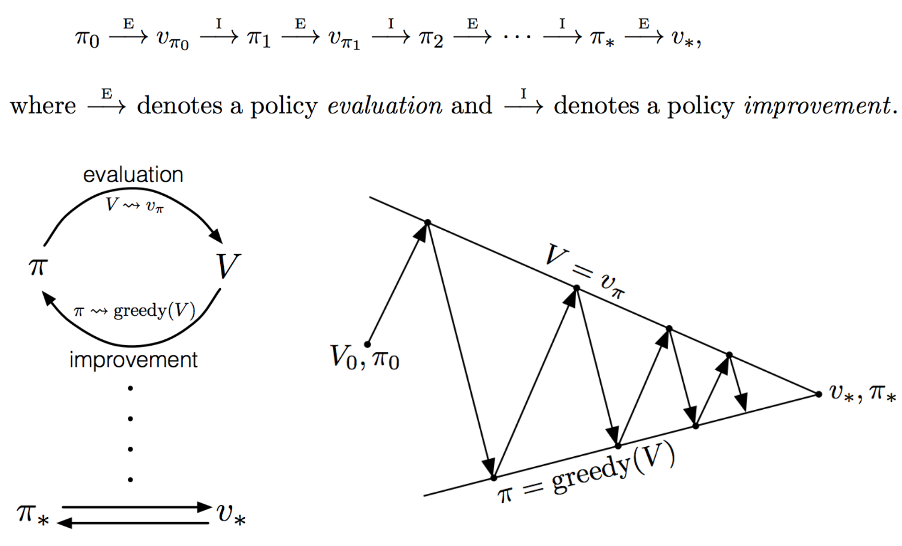
\includegraphics[width=0.9\columnwidth]{images/policy-iteration.png}
    \caption{Illustration of policy iteration}
    \label{fig:policy-iteration}
\end{figure}

Briefly speaking, we initially take a random policy $\pi$, then compute a state-value function $v_{\pi}$ and use $v_{\pi}$ to compute $q_{\pi}$. After that, we select the new greedy policy $\pi'(s)$ from $q_{\pi}$:
$$\pi'(s)= \argmax_a q_{\pi}(s,a)$$

Each policy is guaranteed to be an improvement on the last unless the last policy was already optimal.


\begin{tcolorbox}[title={Policy Iteration (using iterative policy evaluation) for estimating $\pi \approx \pi_*$}]

  \textbf{1. Initialization:} $V(s) \in \mathbb{R}$ and $\pi(s) \in \mathcal{A}(s)$ arbitrarily for all $s \in \mathcal{S}$ \\

  \textbf{2. Policy Evaluation:}
  \begin{description}
      \item $\;\;\;$ \textbf{Loop:}
      \begin{description}
        \item $\;\;\;$ $\Delta \leftarrow 0$
        \item $\;\;\;$ \textbf{Loop for each $s \in \mathcal{S}$:}
        \begin{description}
          \item $\;\;\;$ $v \leftarrow V(s)$
          \item $\;\;\;$ $V(s) \leftarrow \sum_{s', r} p(s',r|s,\pi(s)) [r + \gamma V(s')]$
          \item $\;\;\;$ $\Delta \leftarrow \max (\Delta , | v - V(s) |)$
        \end{description}
      \end{description}
      \textbf{Until:} $\Delta < \theta$ (a small positive number determining the accuracy of estimation)
  \end{description}

  \textbf{3. Policy Improvement:}
  \begin{description}
      \item $\;\;\;$ $policy–stable \leftarrow true$
      \item $\;\;\;$ \textbf{For each $s \in \mathcal{S}$:}
      \begin{description}
        \item $\;\;\;$ $old–action \leftarrow \pi(s)$
        \item $\;\;\;$ $\pi(s) \leftarrow \argmax_a \sum_{s', r} p(s',r | s,a)[r + \gamma V(s')]$
        \item $\;\;\;$ If $old–action \neq \pi(s)$, then $policy–stable \leftarrow false$
      \end{description}
      \item $\;\;\;$ If $policy–stable$, then stop and return $V \approx v_*$ and $\pi \approx \pi_*$; else go to 2
  \end{description}
\end{tcolorbox}



\subsection{Generalized Policy Iteration (GPI)}\label{generalized-policy-iteration}

\textbf{What:} We use the term generalized policy iteration (GPI) to refer to the \uline{general idea of letting \textcolor{blue}{policy evaluation} and \textcolor{blue}{policy improvement} processes interact}, independent of the granularity and other details of the two processes.

\textbf{Why:} Almost all reinforcement learning methods are well described as GPI.


\subsection{Value Iteration}\label{value-iteration}

\textbf{What:} a special case of generalized policy iteration.

\textbf{Why:} It allows us to \uline{\textbf{combine} \textcolor{blue}{policy evaluation} and \textcolor{blue}{policy improvement} into a single update}.


\begin{tcolorbox}[title={Value Iteration, for estimating  $\pi \approx \pi_*$}]

  \textbf{Algorithm parameters:}
  \begin{itemize}
    \item $\theta > 0 \leftarrow$ small threshold determining accuracy of estimation
  \end{itemize}

  \textbf{Initialize:}
  \begin{itemize}
    \item $V(s)$, for all $s \in \mathcal{S}^+$ arbitrarily
    \item $V(terminal) = 0$
  \end{itemize}


  \textbf{Loop:}
  \begin{description}
      \item $\;\;\;$ $\Delta \leftarrow 0$
      \item $\;\;\;$ \textbf{Loop for each $s \in \mathcal{S}$:}
      \begin{description}
        \item $\;\;\;$ $v \leftarrow V(s)$
        \item $\;\;\;$ $V(s) \leftarrow \max_a \sum_{s', r} p(s',r|s,a) [r + \gamma V(s')]$
        \item $\;\;\;$ $\Delta \leftarrow \max (\Delta , | v - V(s) |)$
      \end{description}
  \end{description}
  \textbf{Until:} $\Delta < \theta$ (a small positive number) \\

  \textbf{Output:} a deterministic policy, $\pi \approx \pi_*$, such that:
  \begin{description}
      \item $\;\;\;$ $\pi(s) = \argmax_a \sum_{s',r} p(s',r|s,a)[r+\gamma V(s')]$
  \end{description}
\end{tcolorbox}


We do not run policy evaluation to completion. We perform just one sweep over all the states. After that, we greedify again. We can write this as an update rule $V(s) \leftarrow \max_a \sum_{s', r} p(s',r|s,a) [r + \gamma V(s')]$ which applies directly to the state-value function. The \uline{update does not reference any specific policy, hence the name \textbf{value iteration}}.

\begin{itemize}
  \item \textcolor{Orange}{Instead of updating the value according to a fixed falsey}, \textcolor{blue}{we update using the action that maximizes the current value estimate}.
\end{itemize}



\subsection{Asynchronous Dynamic Programming}\label{asynchronous-dynamic-programming}

\textbf{What:} a special case of generalized policy iteration.

Asynchronous dynamic programming methods give us freedom to update states in any order, they do not perform systematic sweeps.

Asynchronous algorithms can propagate value information quickly through \textbf{selective updates}. This \uline{can sometimes be more efficient than a systematic sweep}.



\subsection{Efficiency of Dynamic Programming}\label{efficiency-of-dynamic-programming}

The \uline{\textbf{key insight of dynamic programming} is that we do not have to treat the evaluation of each state as a separate problem. We can use the other value estimates we have already worked so hard to compute}.

The process of \uline{using the value estimates of successor states to improve our current value estimate is known as \textbf{bootstrapping}}. This \textcolor{Green}{can be much more efficient than (e.g. a Monte Carlo) method that estimates each value independently}.

\begin{figure}[H]
  \centering  % Remember to centre the figure
    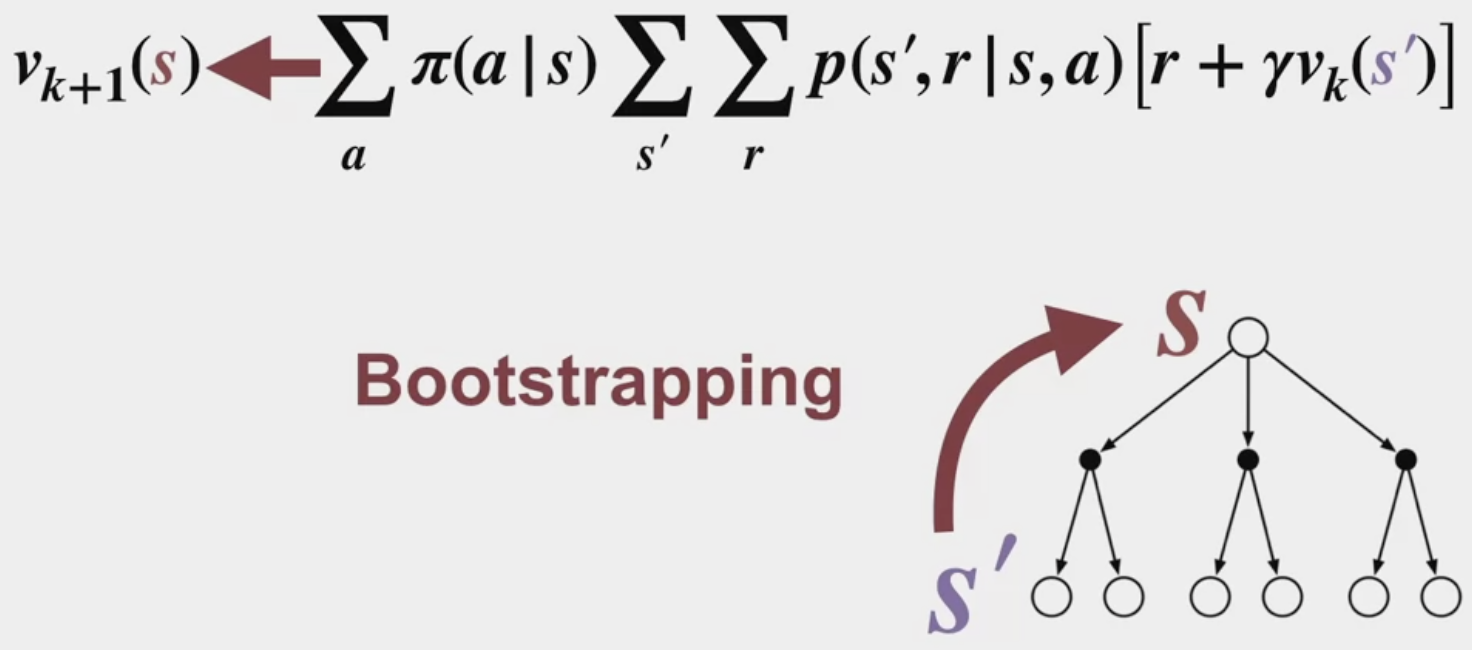
\includegraphics[width=0.8\columnwidth]{images/bootstrapping.png}
    \caption{Illustration of bootstrapping in Dynamic Programming}
    \label{fig:bootstrapping}
\end{figure}











% =============== CHAPTER 5 - Monte Carlo Methods ===============



\section{Monte Carlo Methods}\label{monte-carlo-methods}

\begin{tcolorbox}[colback=yellow!5,colframe=yellow!75!black,title=NOTE]
  To ensure that well-defined returns are available, here we define Monte
  Carlo methods only for \textbf{\colorbox{Yellow}{episodic tasks}}.
  \begin{itemize}
    \item That is, we assume experience is divided into episodes, and that all episodes eventually terminate no matter what actions are selected.
    \item Only on the completion of an episode are value estimates and policies changed.
  \end{itemize}
\end{tcolorbox}

\textbf{What:} sample-based methods for solving reinforcement learning problem.
\begin{itemize}
  \item \textbf{estimating} value functions \(\rightarrow\) \textbf{discovering}
  optimal policies.
\end{itemize}

\textbf{How:} based on \textbf{averaging} \uline{sample returns} \textbf{for
each} \uline{state--action pair}.

\textbf{Pros and cons:}
\begin{itemize}
  \item \textbf{+} Don't require a model (direct access to the environment dynamics)
  \item \textbf{+} Conceptually simple
  \item \textbf{-} Not well suited for step-by-step incremental computation
\end{itemize}

\textbf{Base:}

\begin{itemize}
\item
  Unlike previously, we \textbf{don't assume complete knowledge of the
  environment}.

  \begin{itemize}
  \item
    Unknown transaction dynamics (T) and reward function (r)
  \end{itemize}
\item
  Require only \emph{experience} --- \textbf{sample} sequences of
  \textbf{states, actions, and rewards} from actual or simulated
  interaction with an environment.
\item
  There are \textbf{multiple states}, \emph{each acting like a different
  bandit problem} (like an associative-search or contextual bandit) and
  the different bandit problems are interrelated.
\end{itemize}

\textbf{Terms:}

\begin{itemize}
\item
  The term \textbf{``Monte Carlo''} is often used more broadly for any
  estimation method whose operation involves a significant random
  component.

  \begin{itemize}
  \item
    \textbf{HERE:} Here we use it specifically for methods based on
    averaging complete returns.
  \end{itemize}
\end{itemize}






\subsection{Monte Carlo Prediction}\label{monte-carlo-prediction}

Monte Carlo methods for learning the state-value function for a given
policy.

The \textbf{first-visit MC method} (focus of this chapter) estimates
\(v_\pi(s)\) as the average of the returns following first visits to s,
whereas the \textbf{every-visit MC method} averages the returns
following all visits to s.

\end{document}
